\subsection{GridLAB-D Model Validation}
\textbf{THIS SECTION AND FORWARD NEEDS TO BE REWRITTEN AND EXPLAINED. FOR NOW, I'M POSTING IMAGES HERE TO PRESENT IN THE TECH MEETING}
\newpage
\subsubsection{HPWH Water Demand Behavior}
\begin{figure}[H]
    \centering
    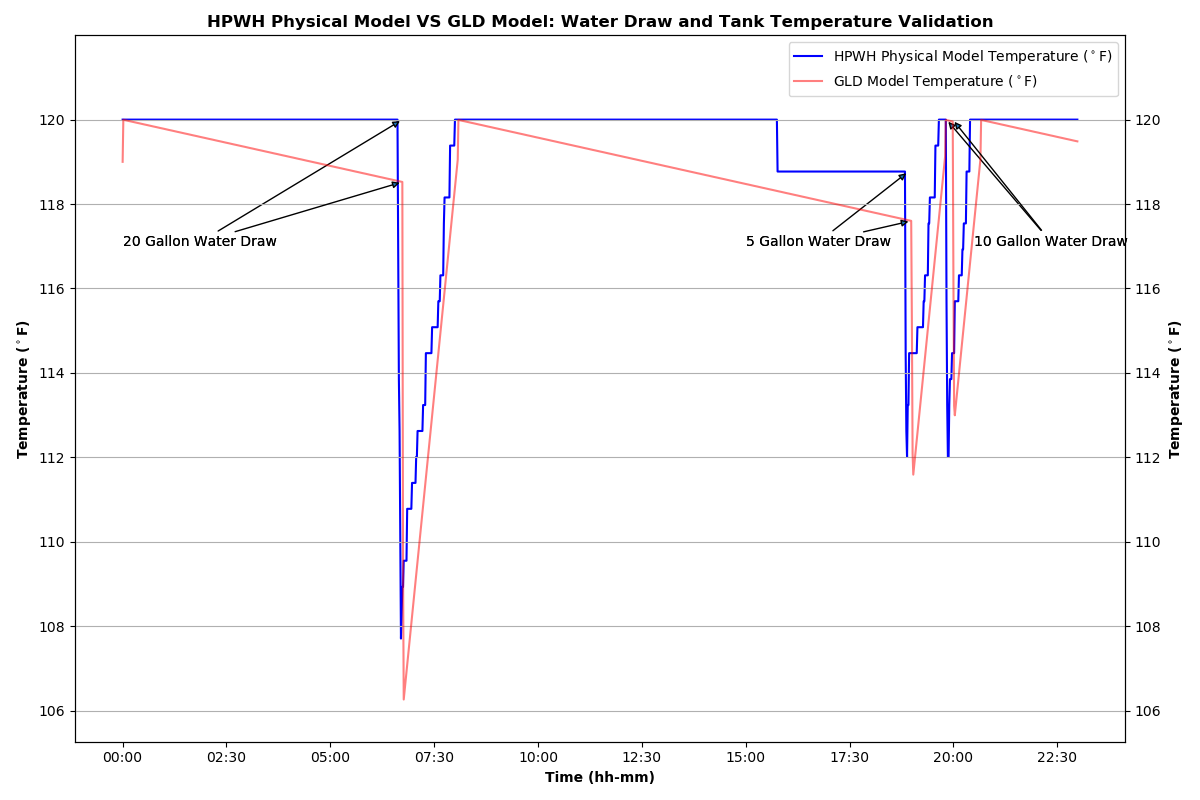
\includegraphics[width=1.1\columnwidth]{Pictures/Temperature_validation.png}
    \caption{GLD and Physical Model Validation: Water Draw Validation}
    %\label{fig:temp_data}
\end{figure}

\newpage
\subsubsection{Idle Losses}
\begin{figure}[H]
    \centering
    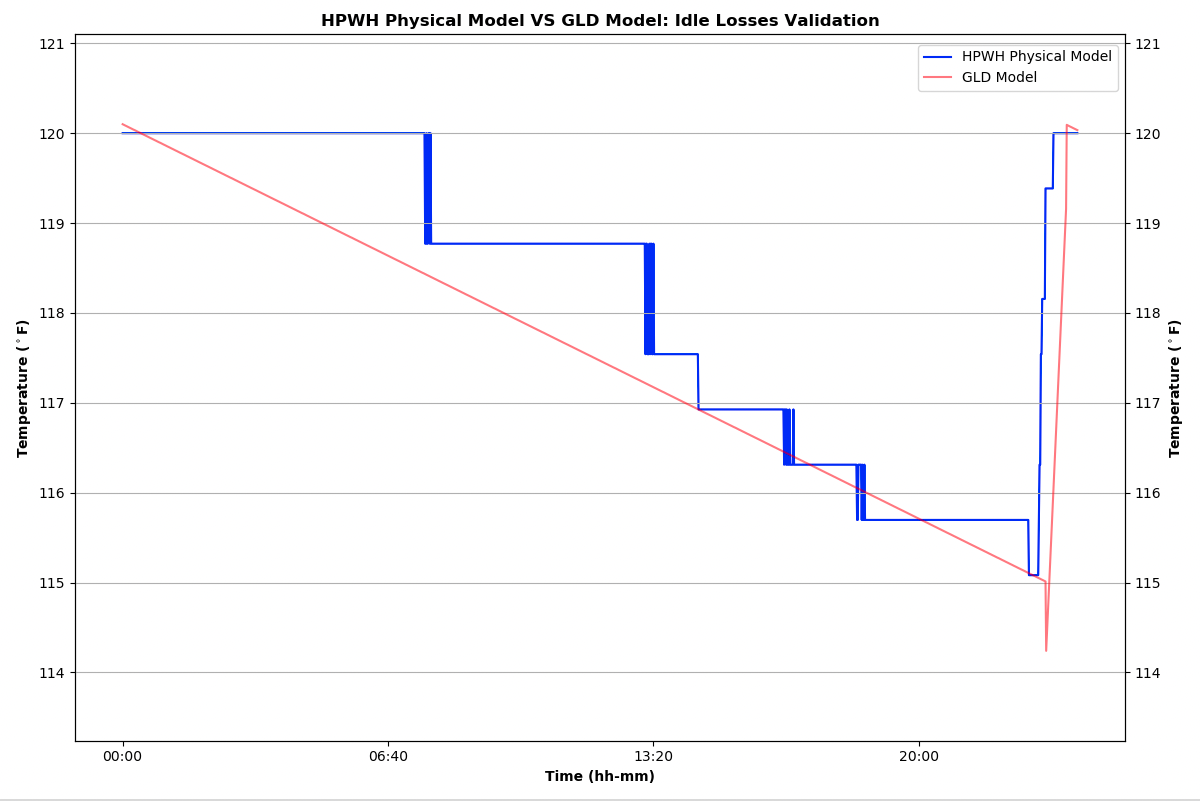
\includegraphics[width=1.1\columnwidth]{Pictures/idle_losses.png}
    \caption{GLD and Physical Model Validation: Idle Losses}
    %\label{fig:temp_data}
\end{figure}

\newpage
\subsubsection{Heating Sources Switching}
\begin{figure}[H]
    \centering
    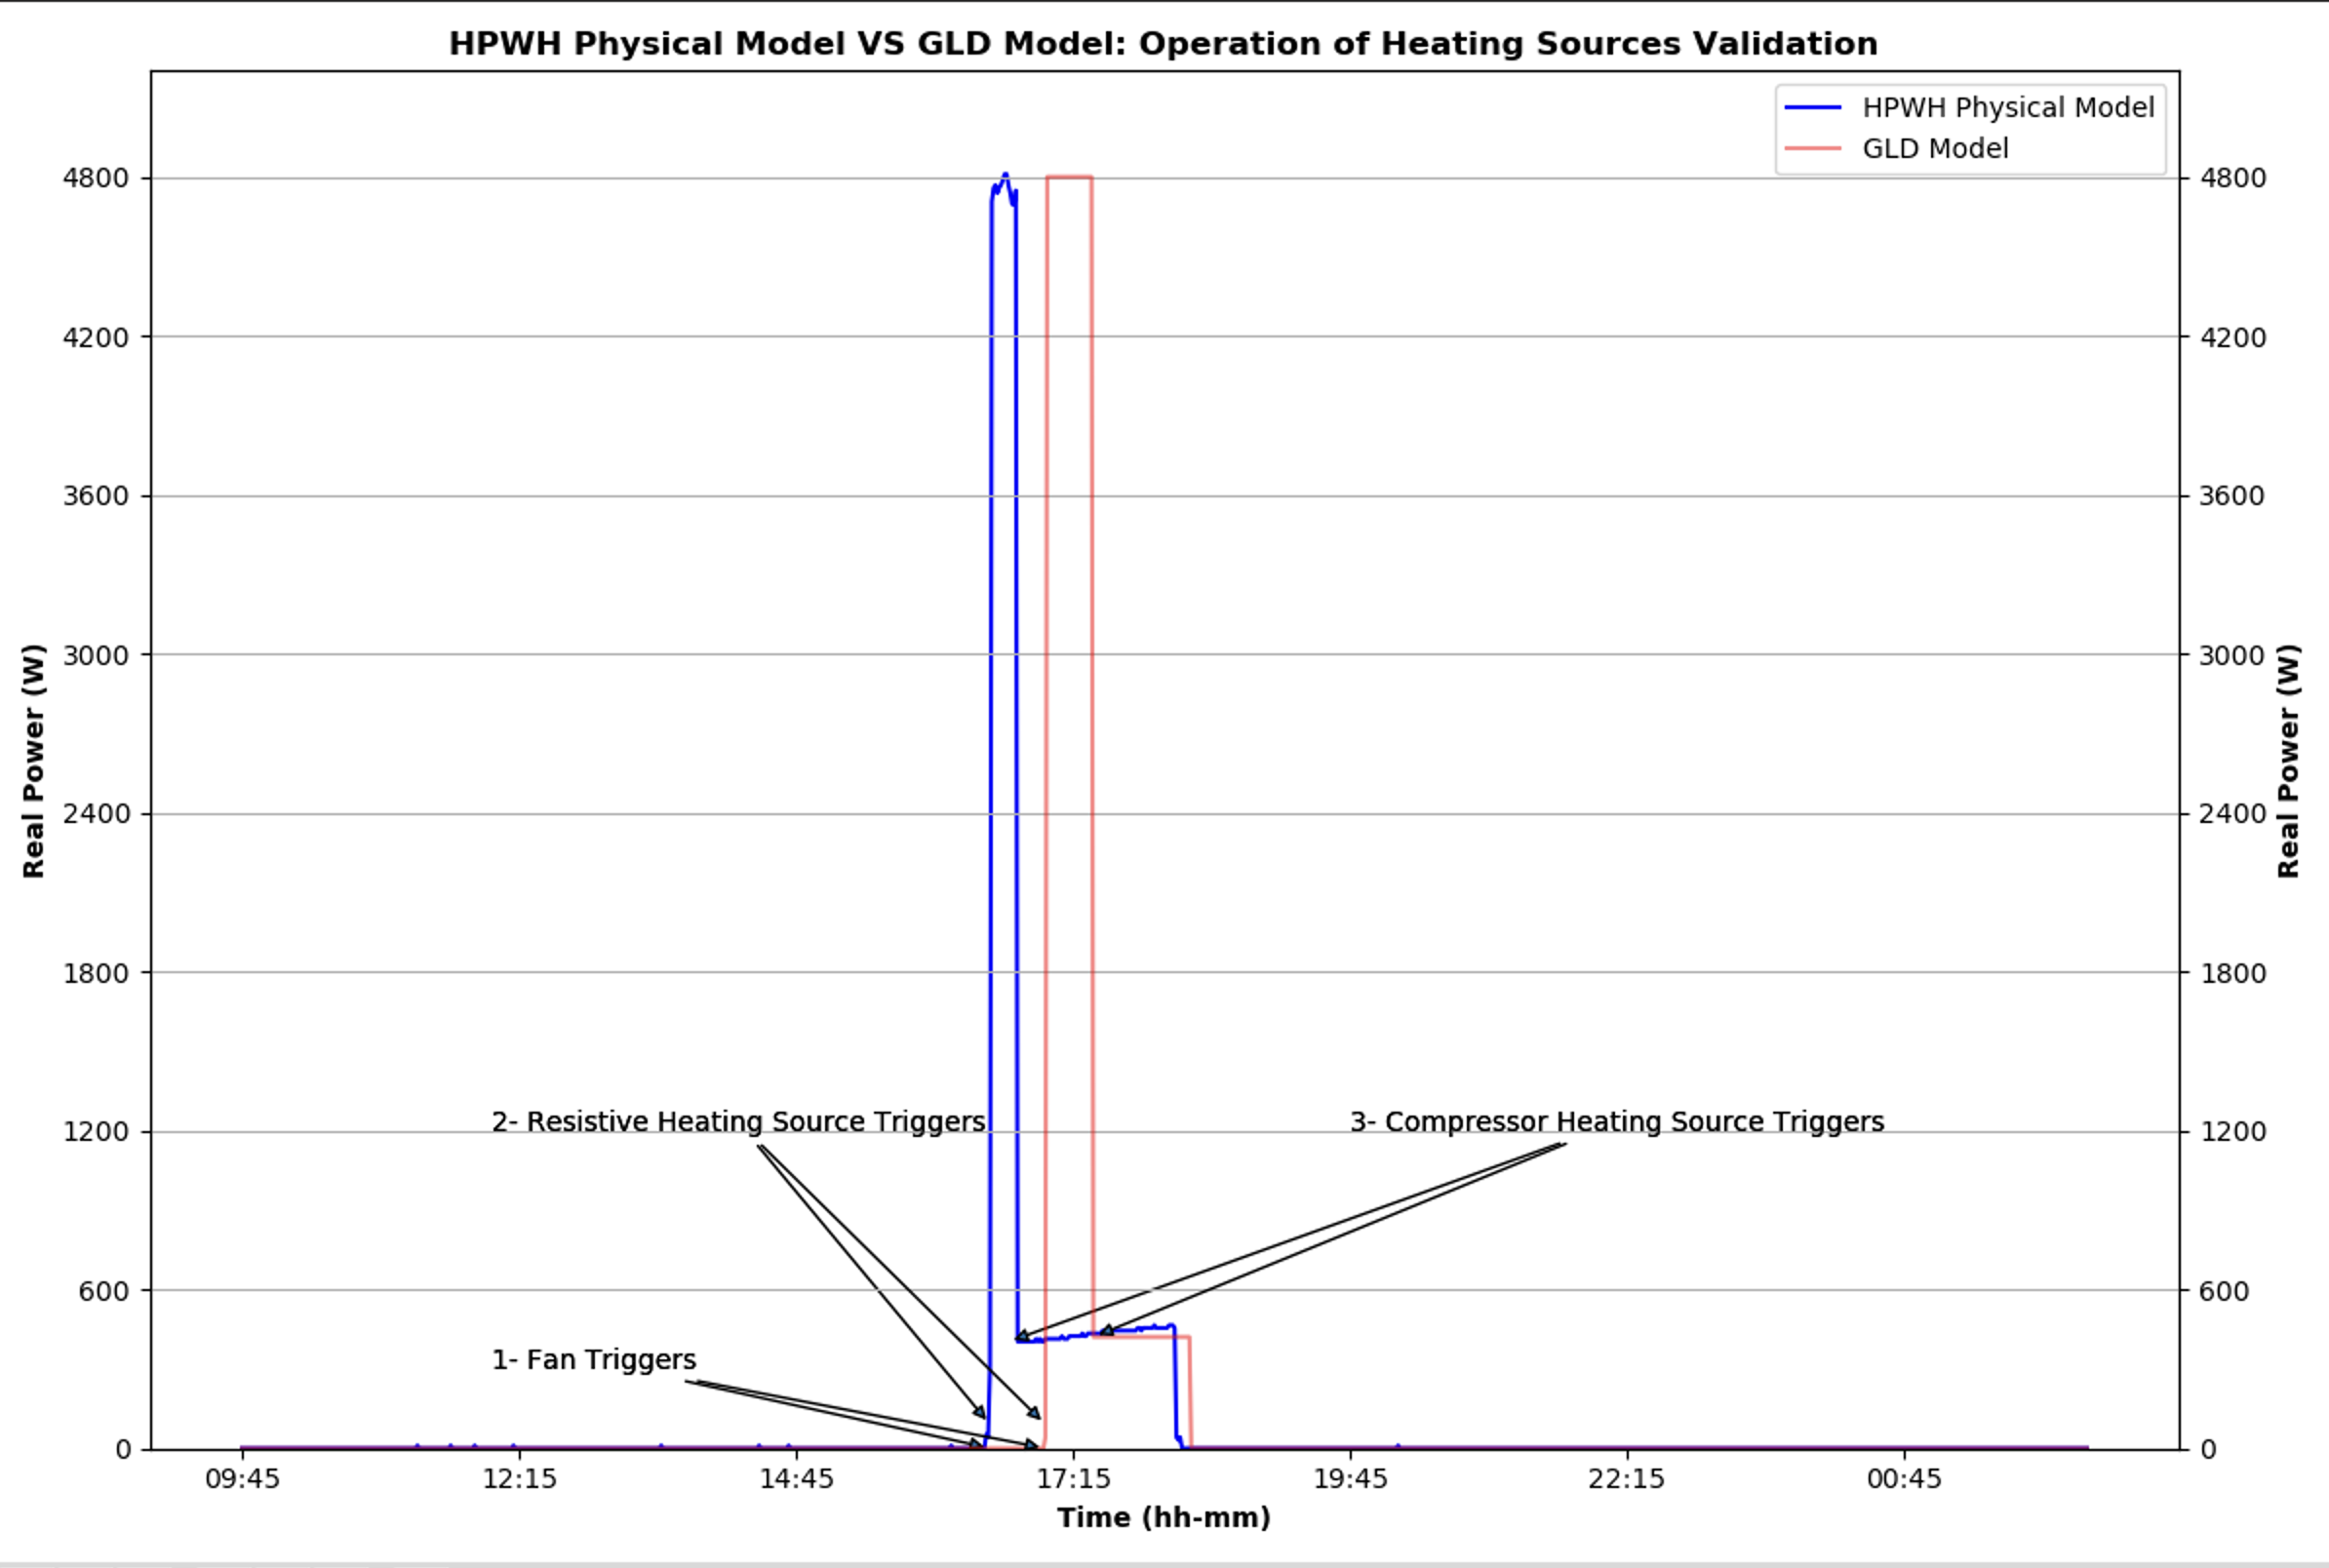
\includegraphics[width=1.1\columnwidth]{Pictures/heating_element_switching.png}
    \caption{GLD and Physical Model Validation: Heating Sources Switching}
    %\label{fig:temp_data}
\end{figure}
\newpage
\subsubsection{Data Samples}
\begin{figure}[H]
    \centering
    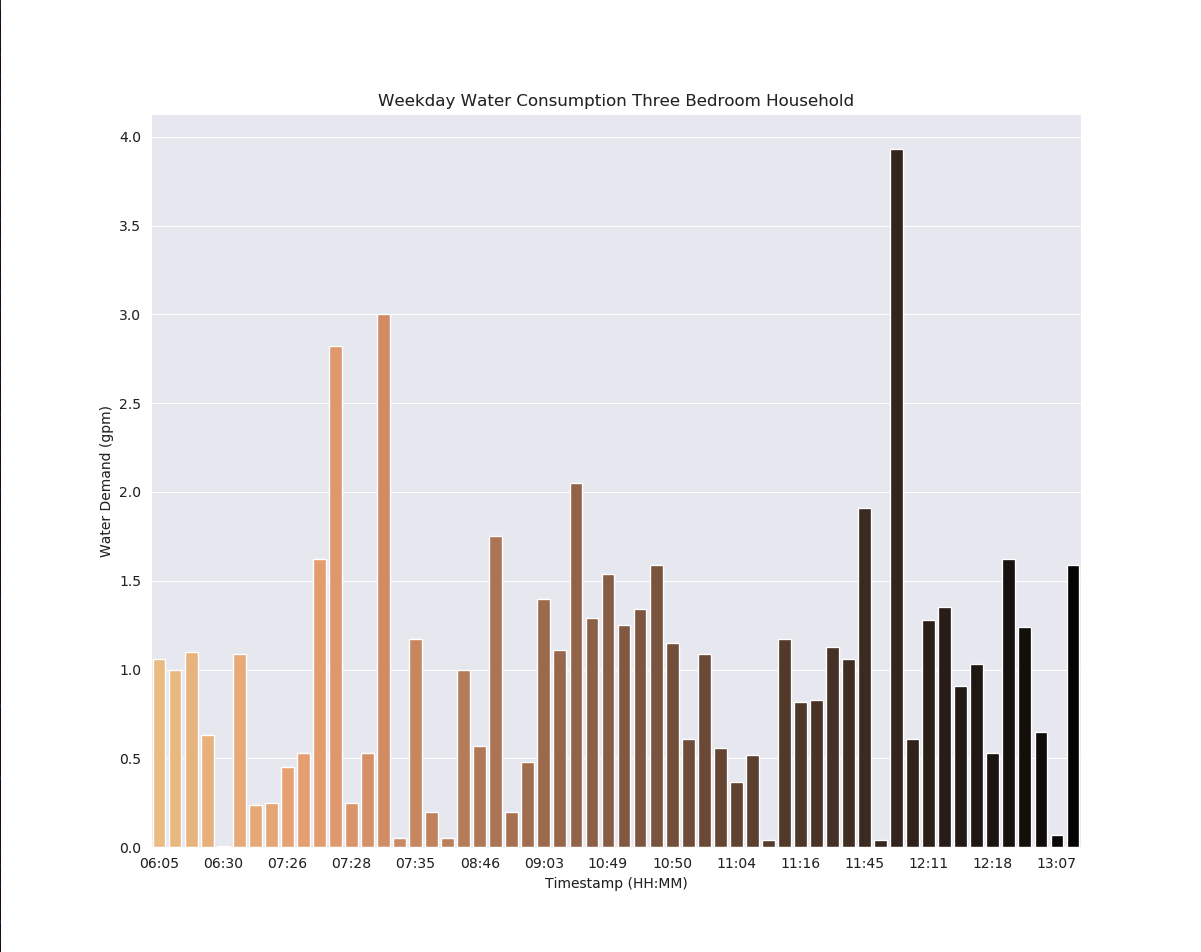
\includegraphics[width=1.1\columnwidth]{Pictures/water_demand_sample.png}
    \caption{Water Demand Sample}
    %\label{fig:temp_data}
\end{figure}

\newpage

\begin{figure}[H]
    \centering
    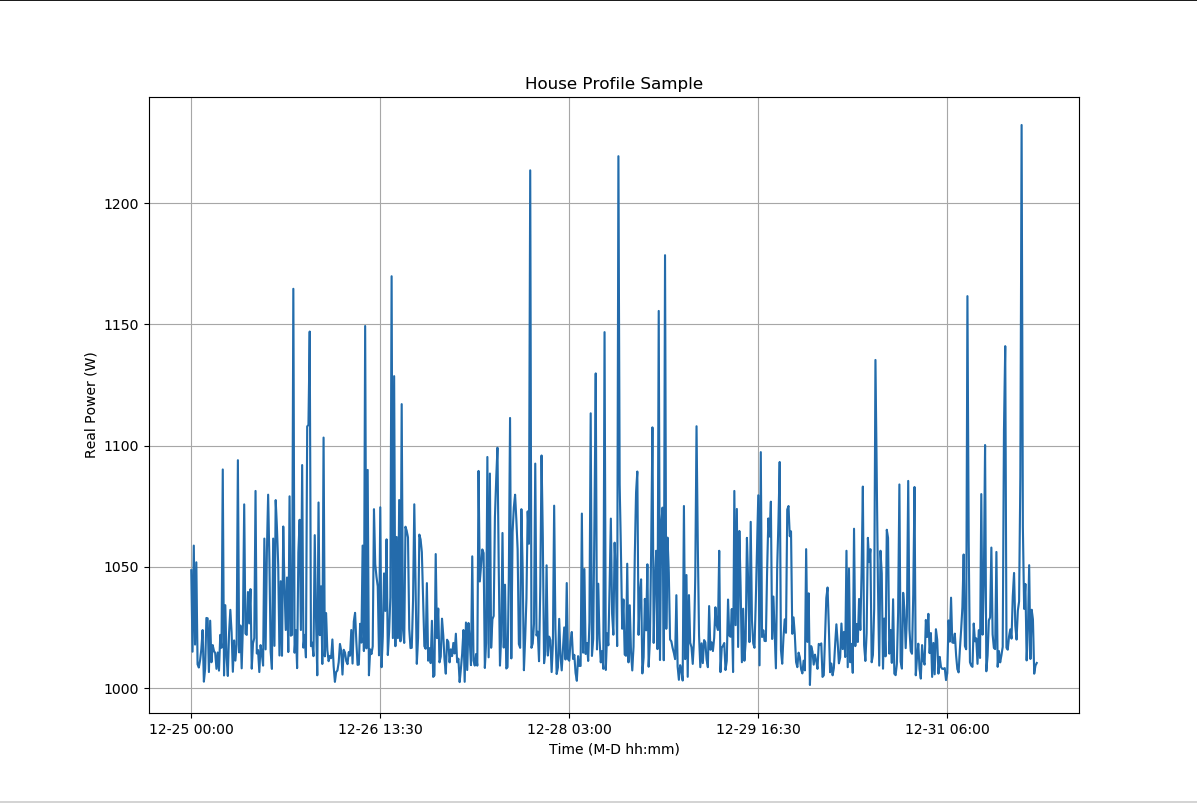
\includegraphics[width=1.1\columnwidth]{Pictures/house_profile_sample.png}
    \caption{ }
    %\label{fig:temp_data}
\end{figure}

\newpage

// ==================================================================================

\begin{figure}[H]
    \centering
    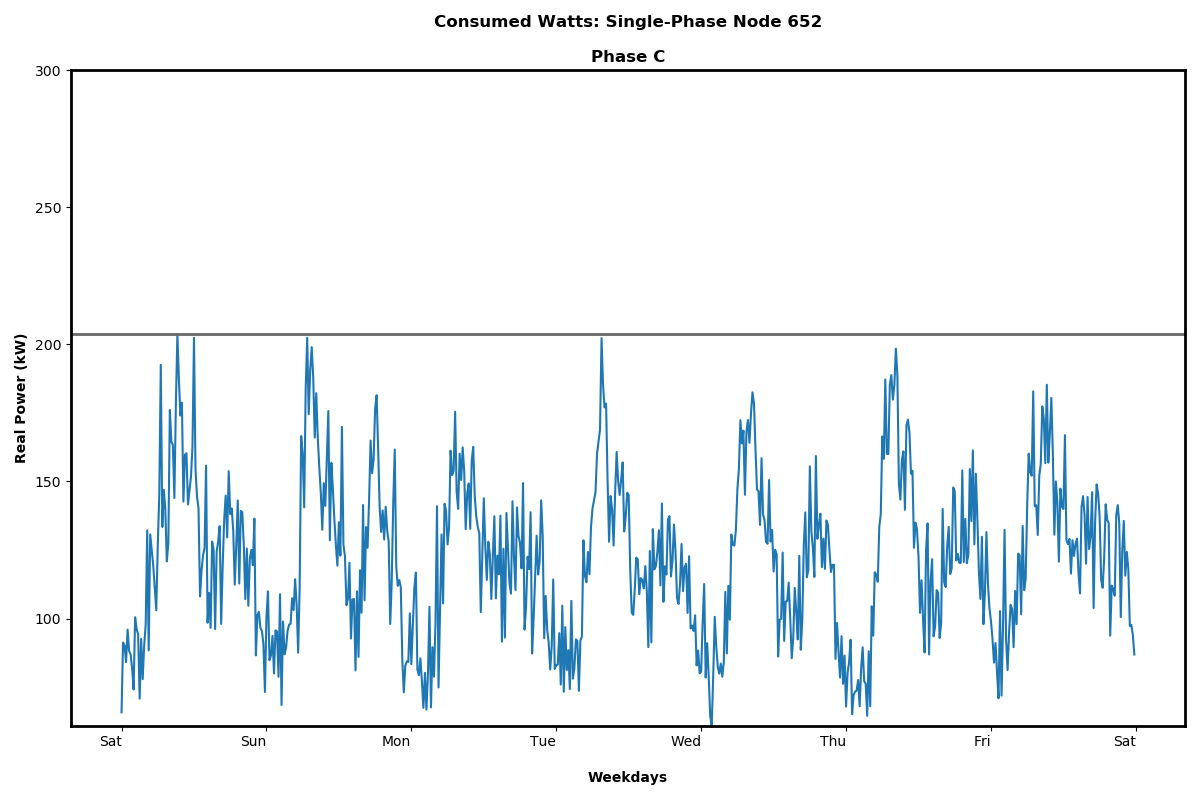
\includegraphics[width=1.1\columnwidth]{Pictures/basecase_single_phase_652_power.png}
    \caption{ }
    %\label{fig:basecase_pow}
\end{figure}

\newpage

\begin{figure}[H]
    \centering
    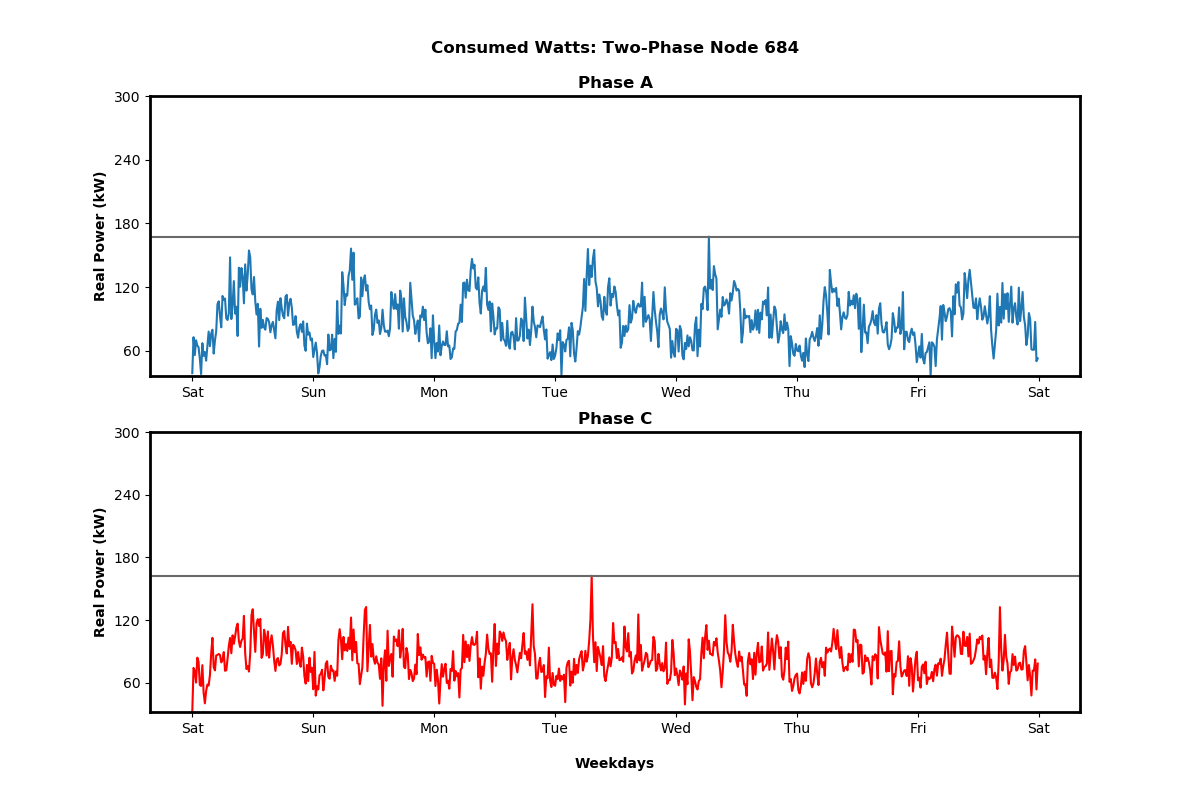
\includegraphics[width=1.1\columnwidth]{Pictures/basecase_two_phase_684_power.png}
    \caption{ }
    %\label{fig:temp_data}
\end{figure}

\newpage

\begin{figure}[H]
    \centering
    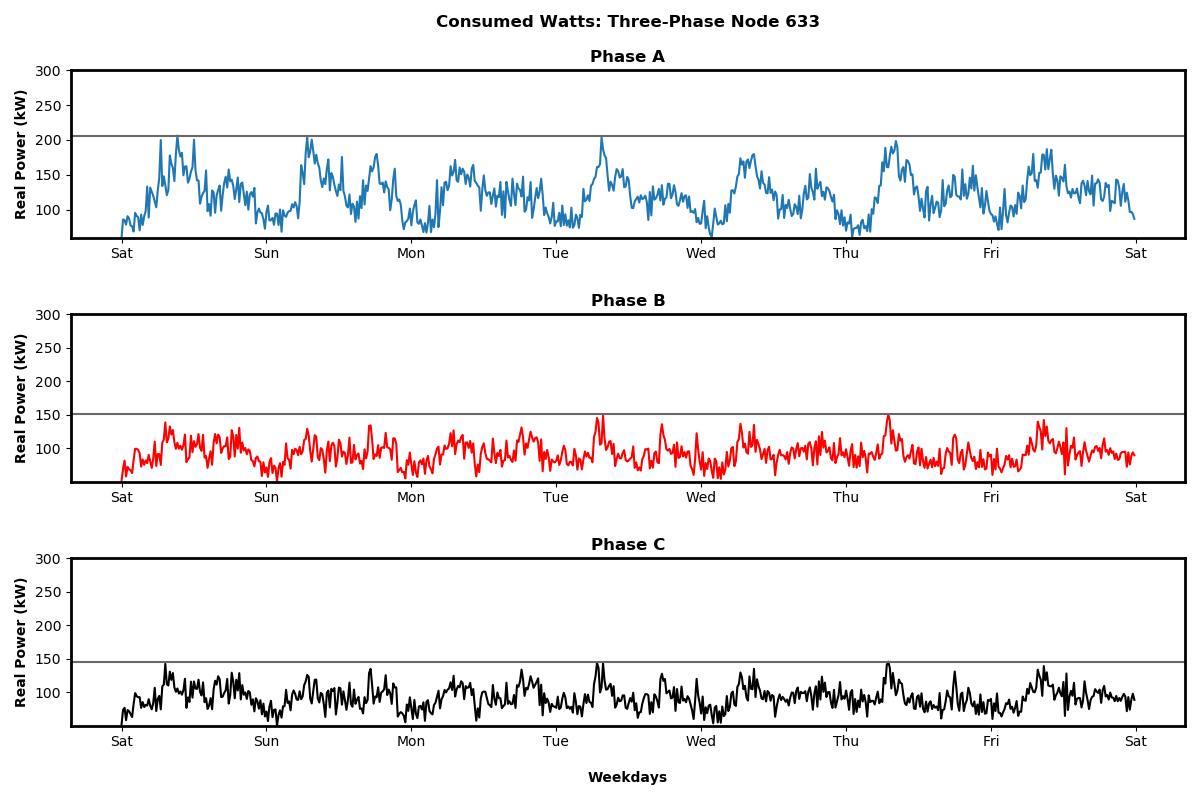
\includegraphics[width=1.1\columnwidth]{Pictures/basecase_three_phase_633_power.png}
    \caption{ }
    %\label{fig:temp_data}
\end{figure}
\newpage


\begin{figure}[H]
    \centering
    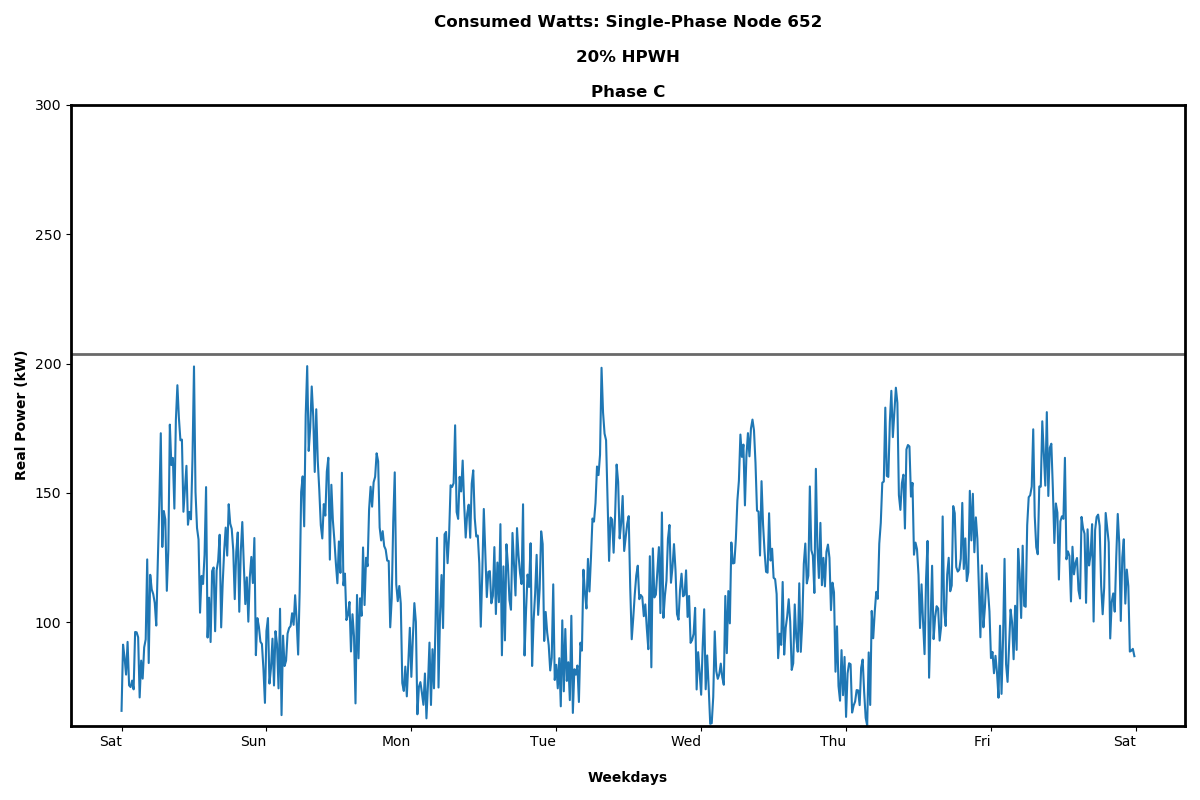
\includegraphics[width=1.1\columnwidth]{Pictures/twenty_single_phase_652_power.png}
    \caption{ }
    %\label{fig:basecase_pow}
\end{figure}

\newpage

\begin{figure}[H]
    \centering
    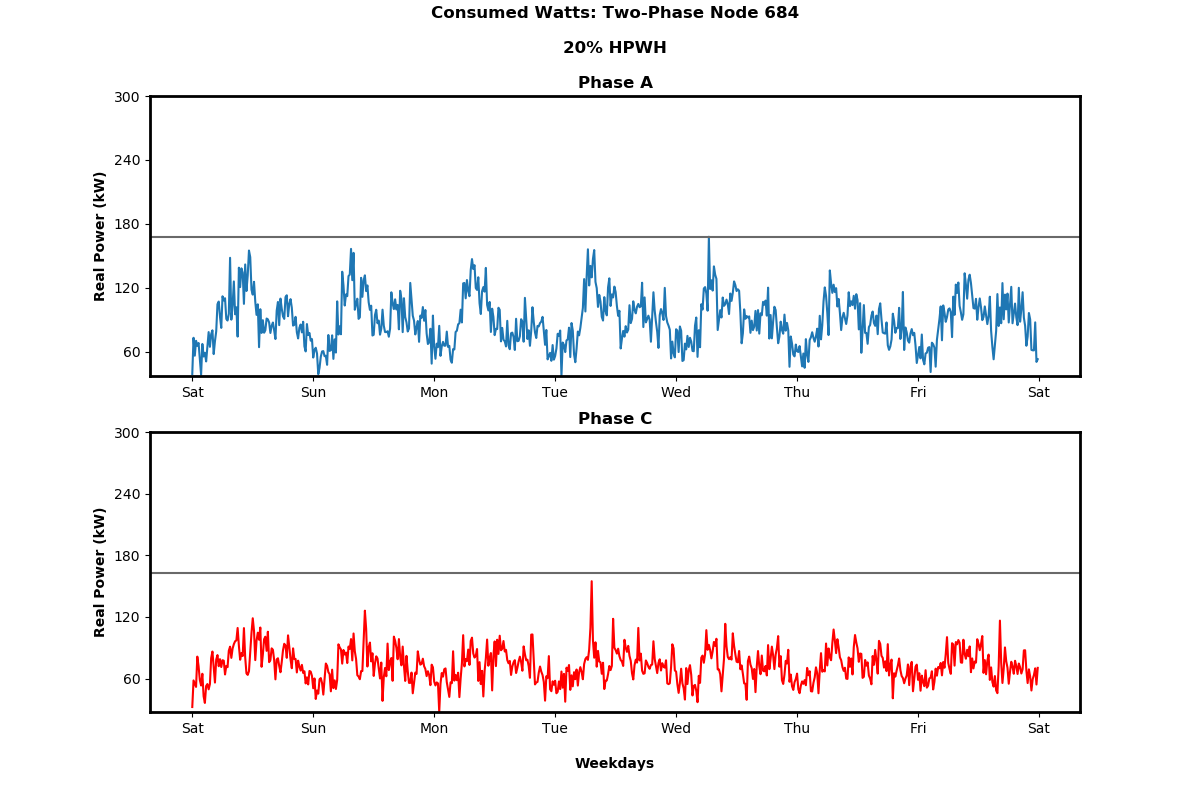
\includegraphics[width=1.1\columnwidth]{Pictures/twenty_two_phase_684_power.png}
    \caption{ }
    %\label{fig:temp_data}
\end{figure}

\newpage

\begin{figure}[H]
    \centering
    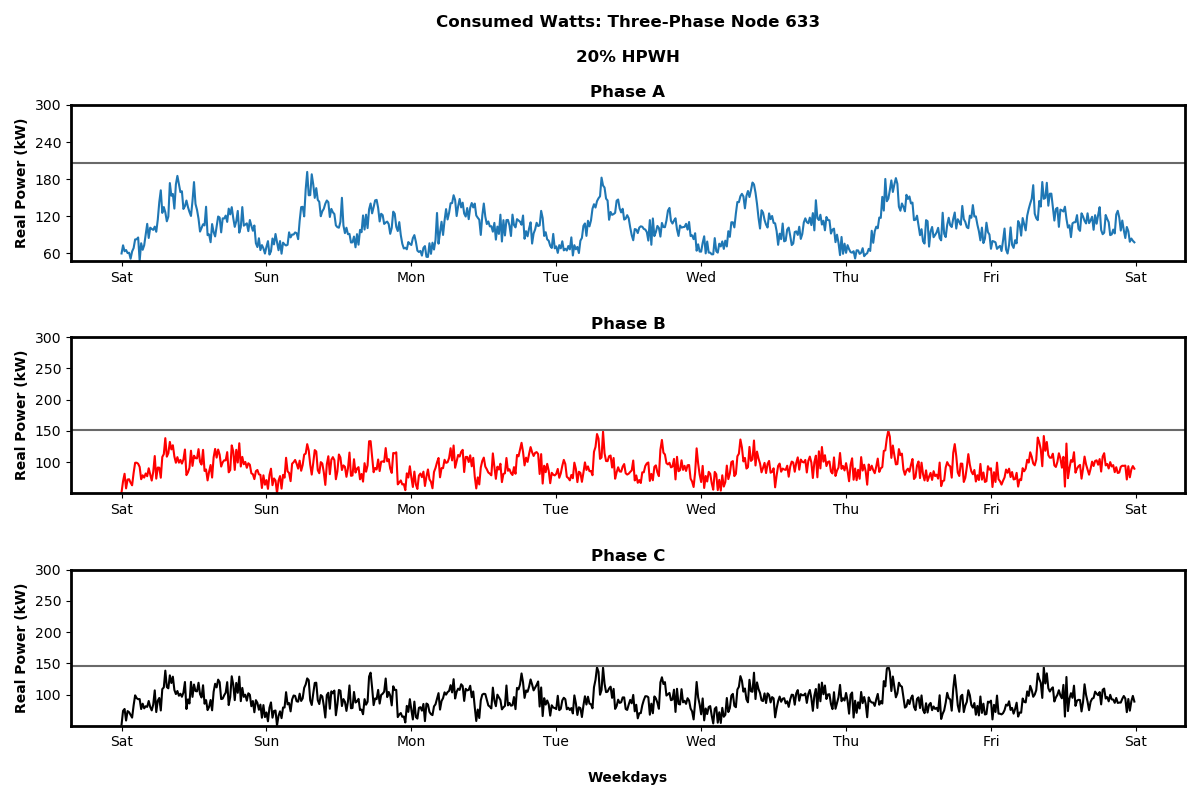
\includegraphics[width=1.1\columnwidth]{Pictures/twenty_three_phase_633_power.png}
    \caption{ }
    %\label{fig:temp_data}
\end{figure}




\begin{figure}[H]
    \centering
    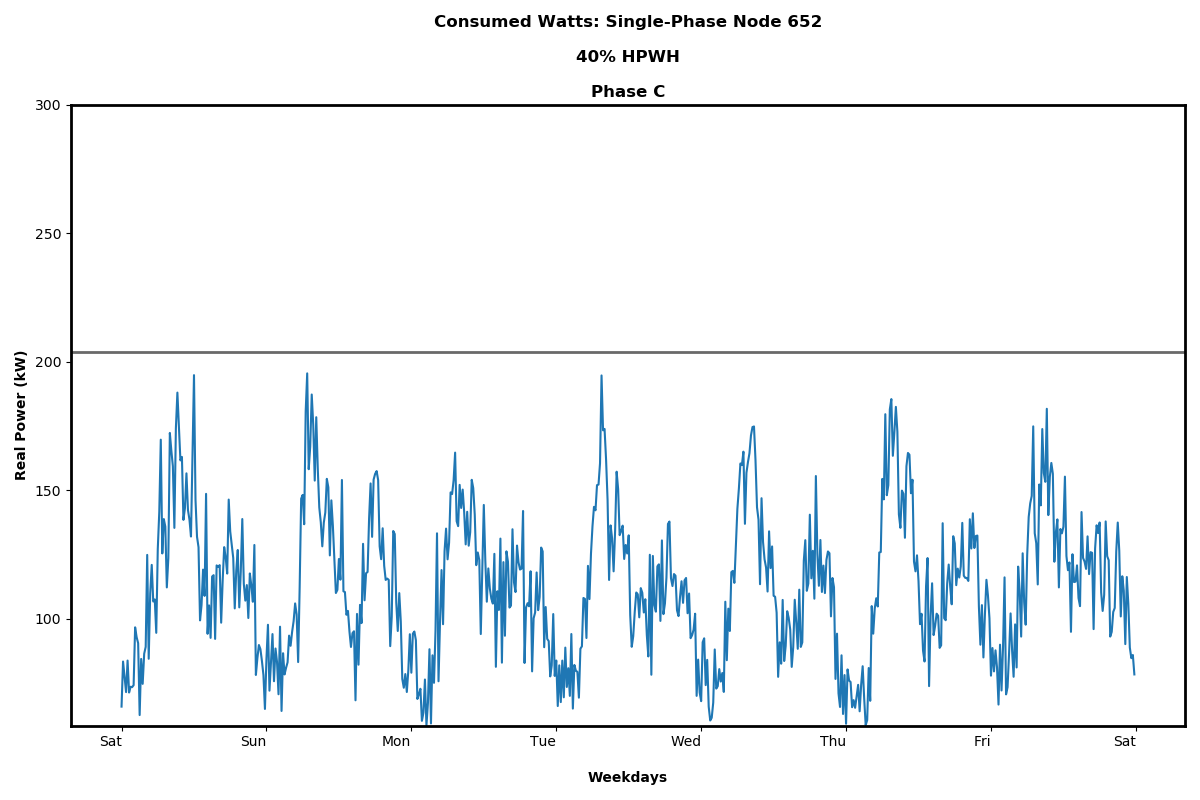
\includegraphics[width=1.1\columnwidth]{Pictures/fourty_single_phase_652_power.png}
    \caption{ }
    %\label{fig:basecase_pow}
\end{figure}

\newpage

\begin{figure}[H]
    \centering
    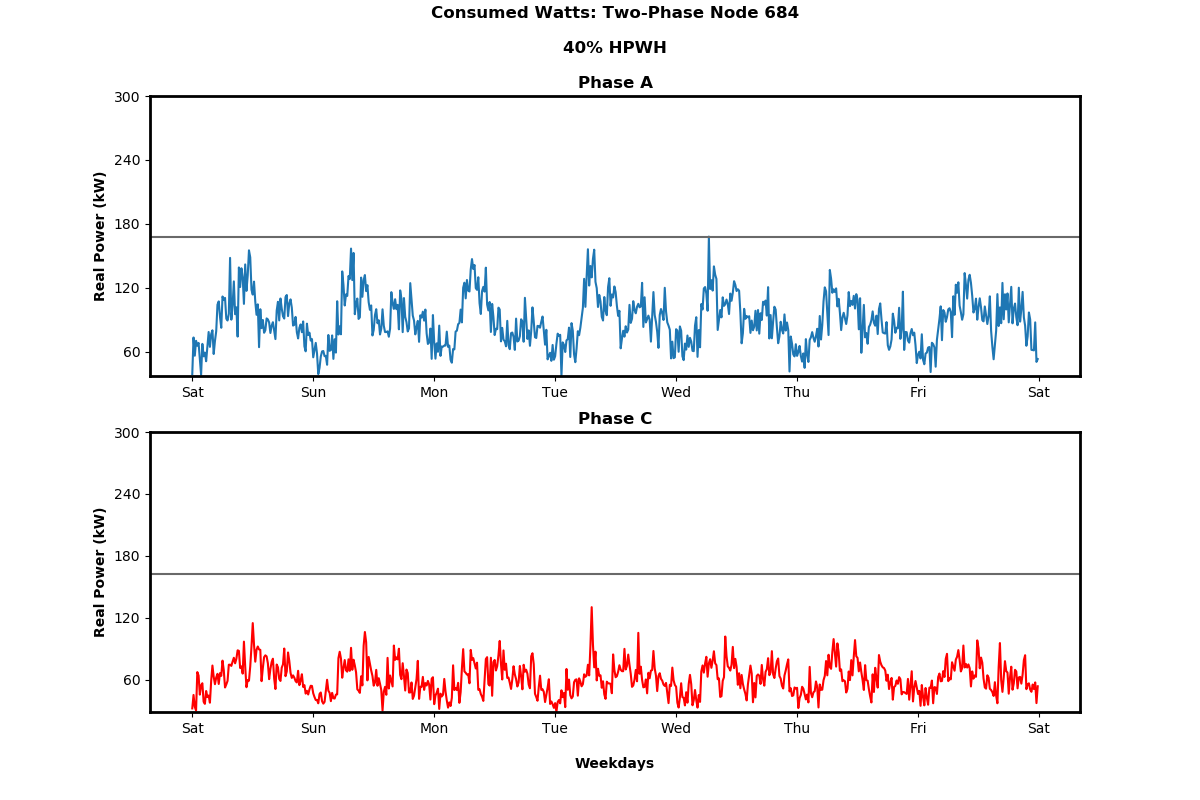
\includegraphics[width=1.1\columnwidth]{Pictures/fourty_two_phase_684_power.png}
    \caption{ }
    %\label{fig:temp_data}
\end{figure}

\newpage

\begin{figure}[H]
    \centering
    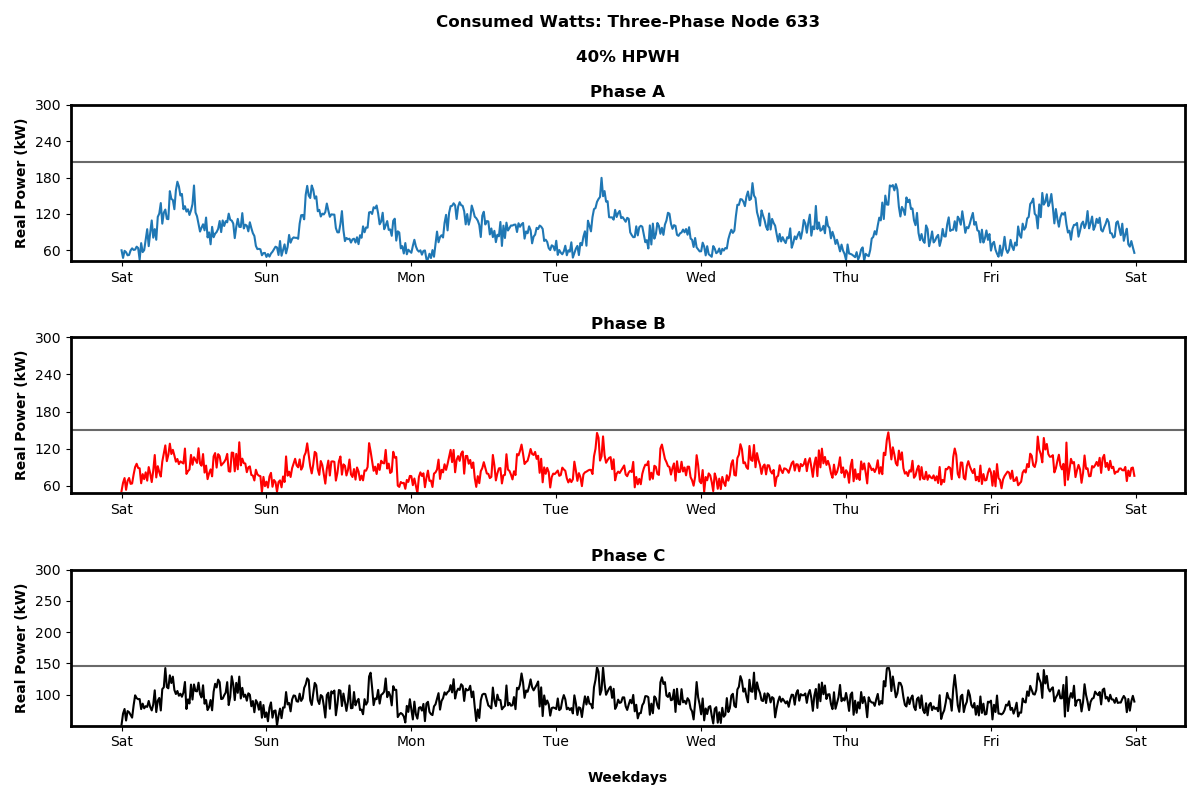
\includegraphics[width=1.1\columnwidth]{Pictures/fourty_three_phase_633_power.png}
    \caption{ }
    %\label{fig:temp_data}
\end{figure}

\newpage



\begin{figure}[H]
    \centering
    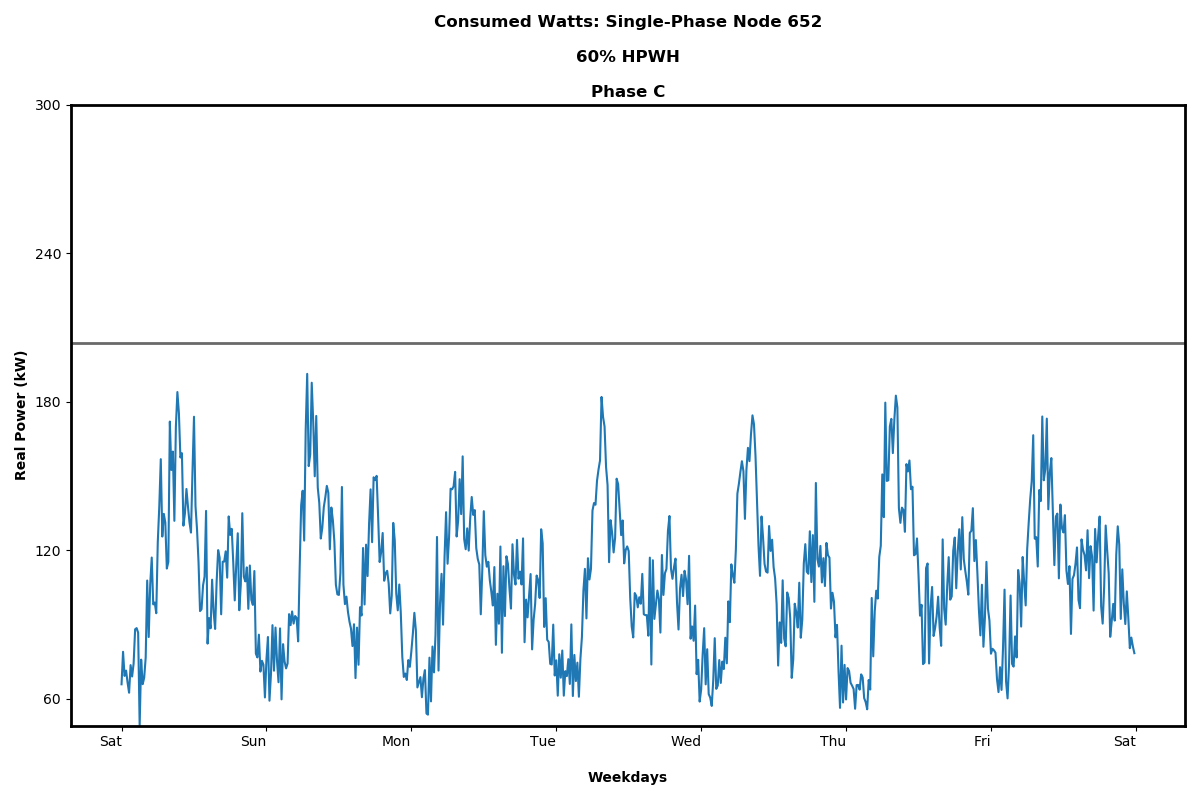
\includegraphics[width=1.1\columnwidth]{Pictures/sixty_single_phase_652_power.png}
    \caption{ }
    %\label{fig:basecase_pow}
\end{figure}

\newpage

\begin{figure}[H]
    \centering
    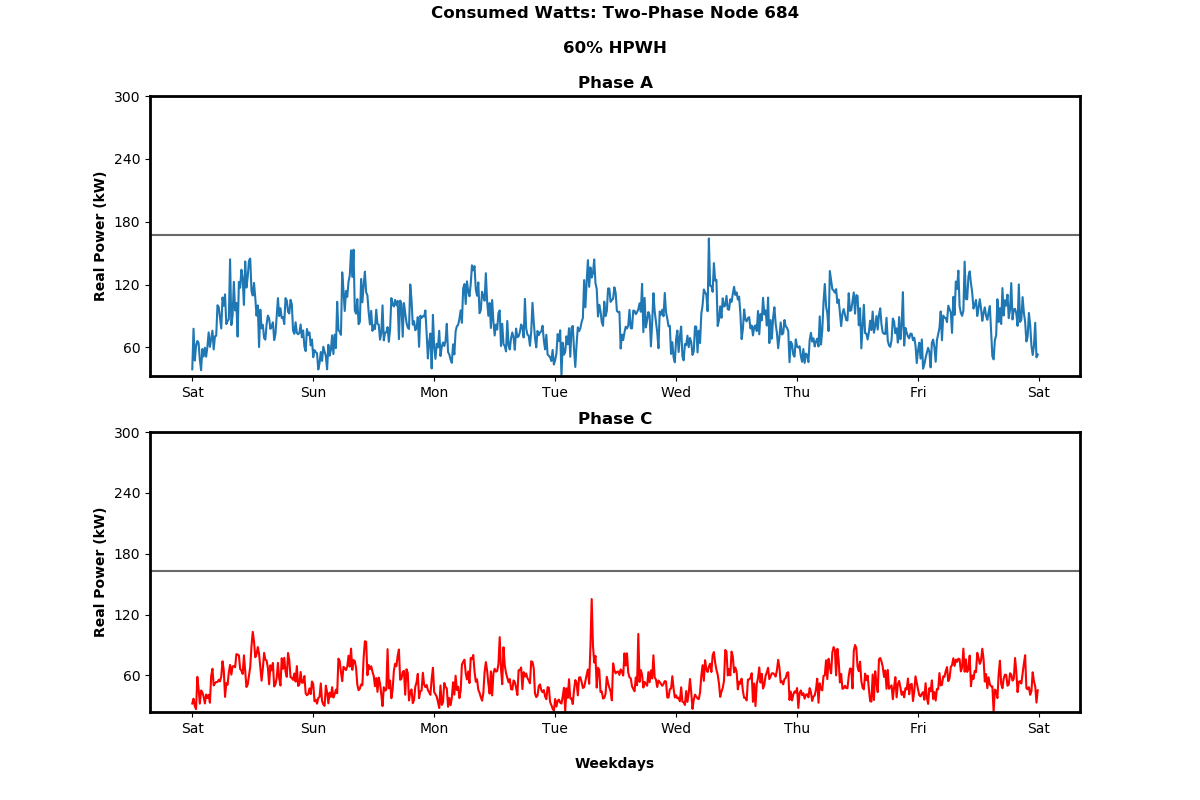
\includegraphics[width=1.1\columnwidth]{Pictures/sixty_two_phase_684_power.png}
    \caption{ }
    %\label{fig:temp_data}
\end{figure}

\newpage

\begin{figure}[H]
    \centering
    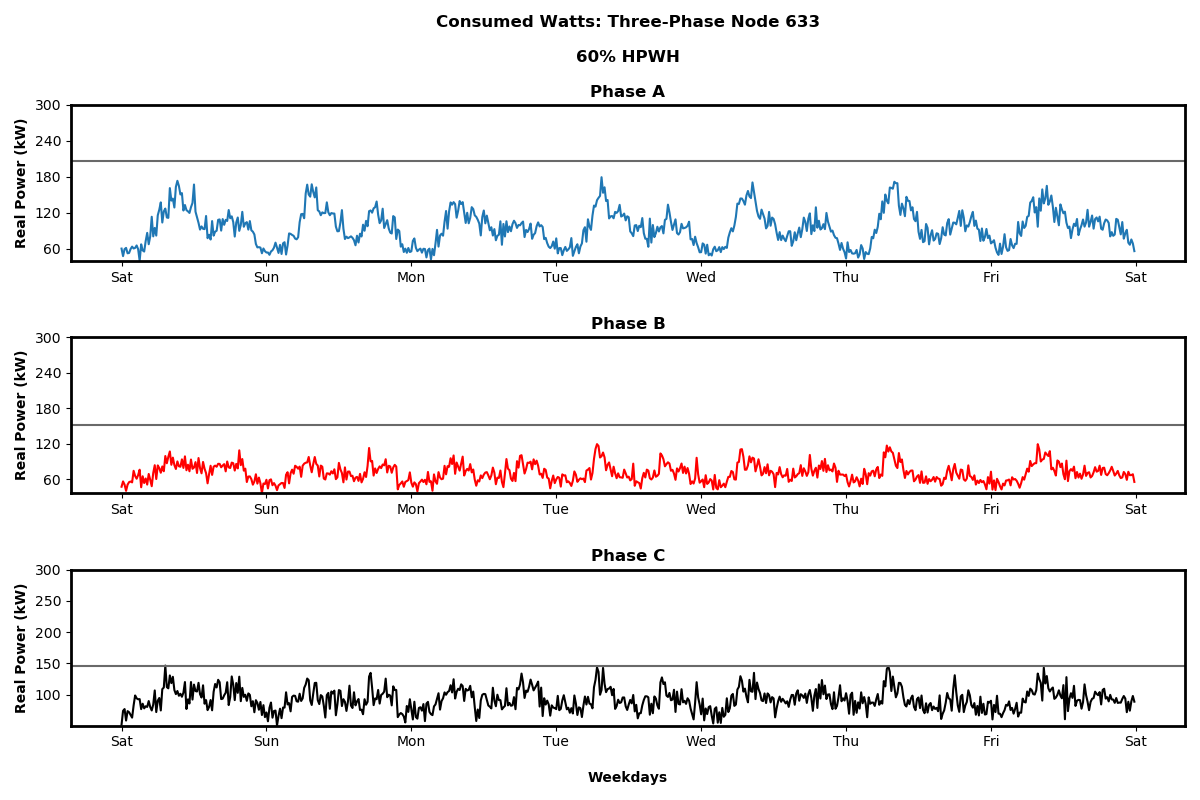
\includegraphics[width=1.1\columnwidth]{Pictures/sixty_three_phase_633_power.png}
    \caption{ }
    %\label{fig:temp_data}
\end{figure}
\newpage





\begin{figure}[H]
    \centering
    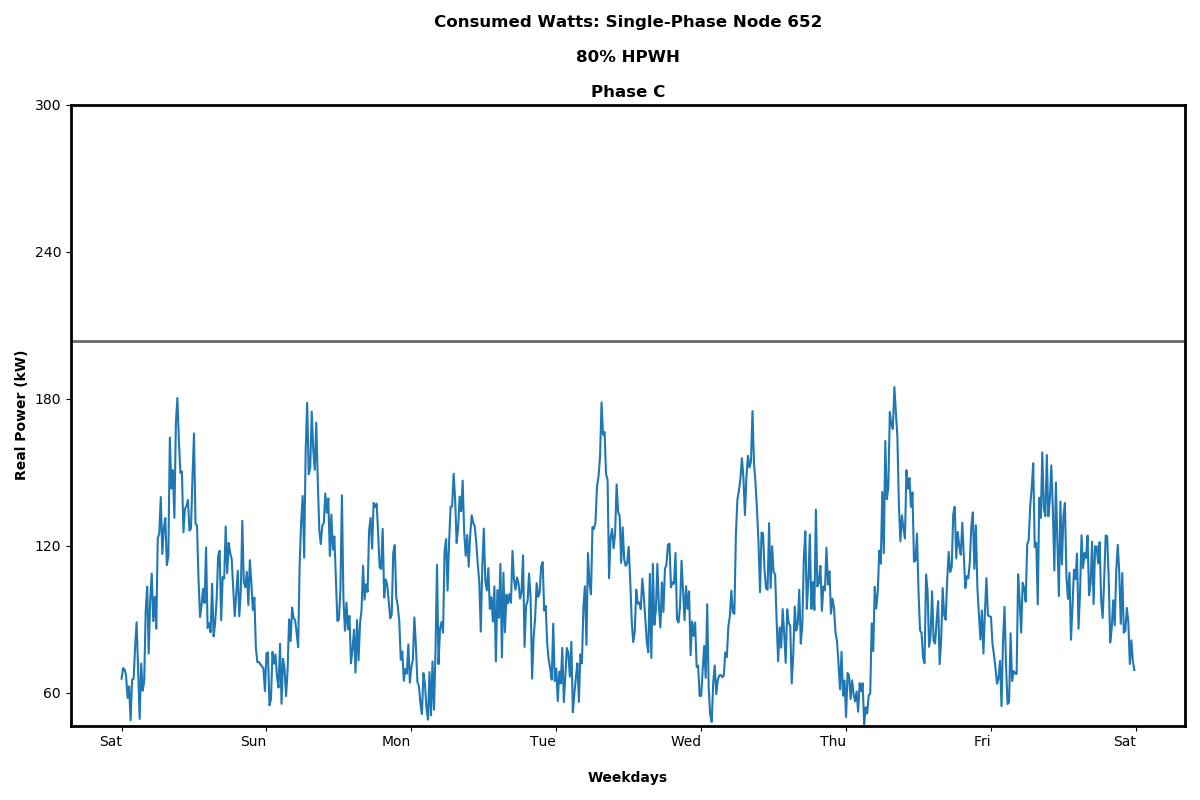
\includegraphics[width=1.1\columnwidth]{Pictures/eighty_single_phase_652_power.png}
    \caption{ }
    %\label{fig:basecase_pow}
\end{figure}

\newpage

\begin{figure}[H]
    \centering
    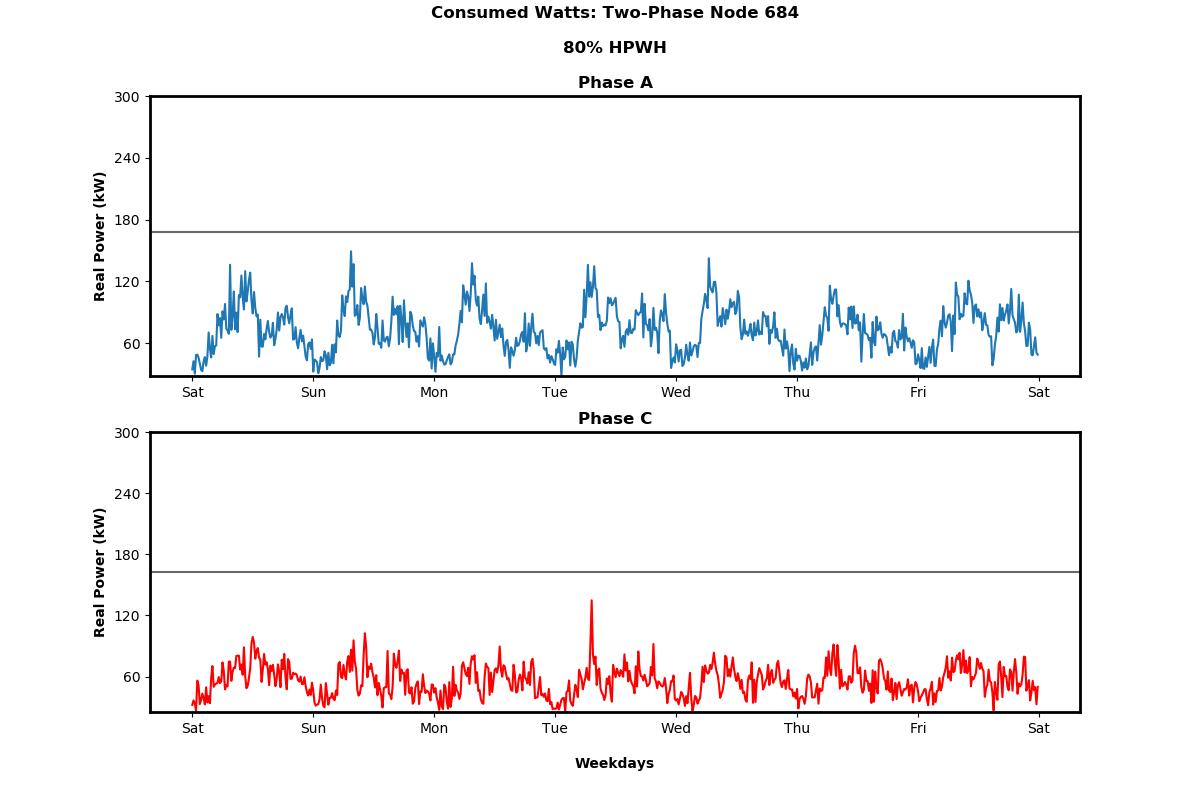
\includegraphics[width=1.1\columnwidth]{Pictures/eighty_two_phase_684_power.png}
    \caption{ }
    %\label{fig:temp_data}
\end{figure}

\newpage

\begin{figure}[H]
    \centering
    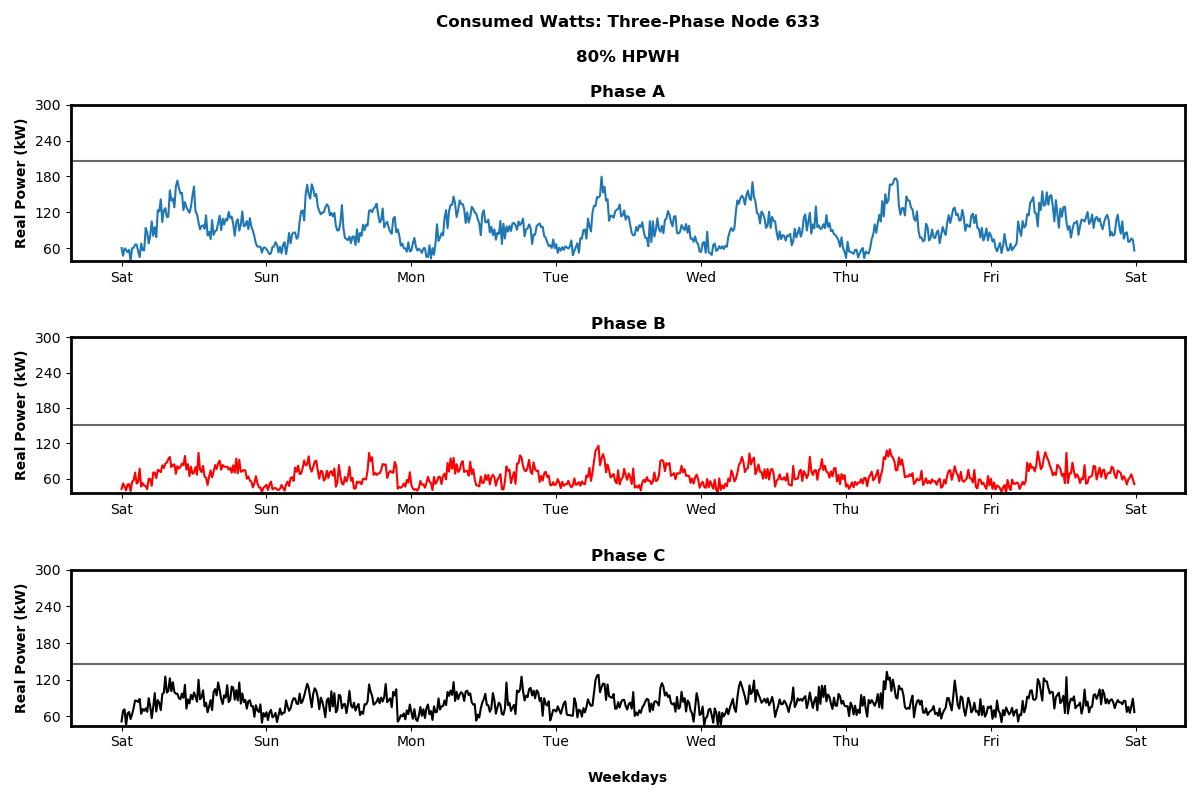
\includegraphics[width=1.1\columnwidth]{Pictures/eighty_three_phase_633_power.png}
    \caption{ }
    %\label{fig:temp_data}
\end{figure}

\newpage





\begin{figure}[H]
    \centering
    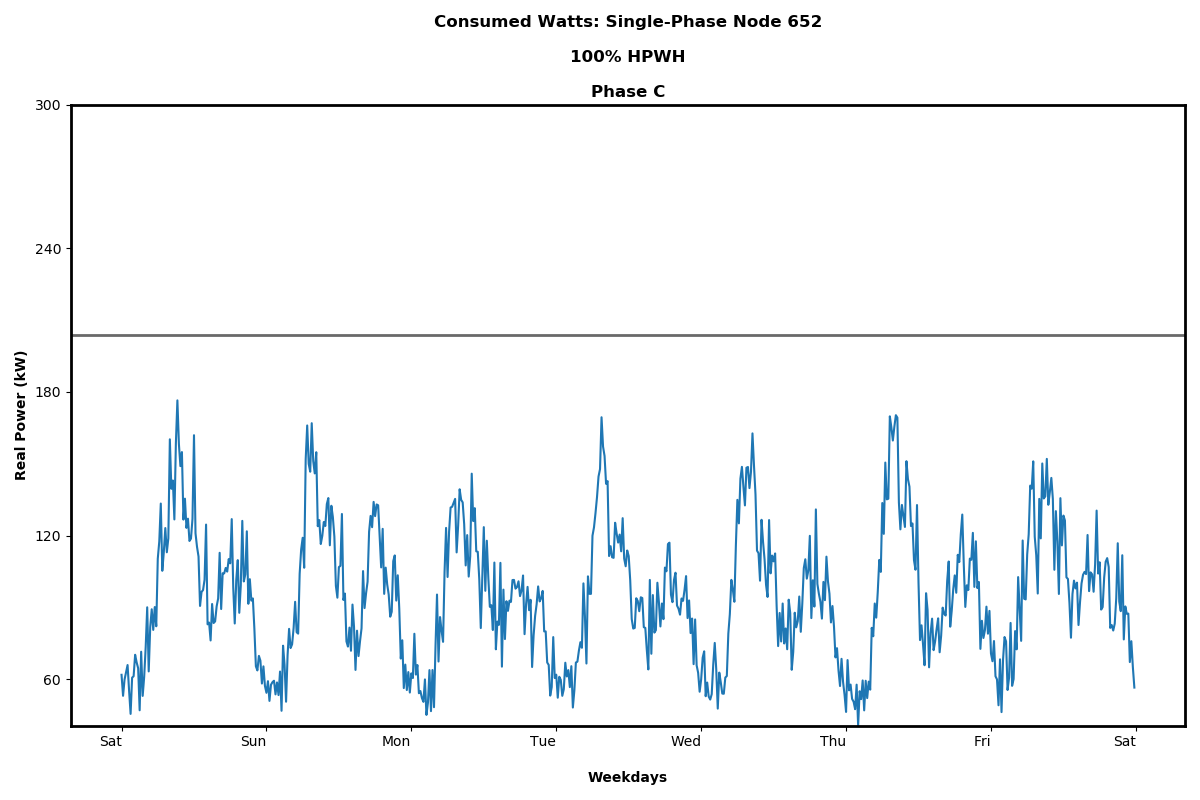
\includegraphics[width=1.1\columnwidth]{Pictures/hundred_single_phase_652_power.png}
    \caption{ }
    %\label{fig:basecase_pow}
\end{figure}

\newpage

\begin{figure}[H]
    \centering
    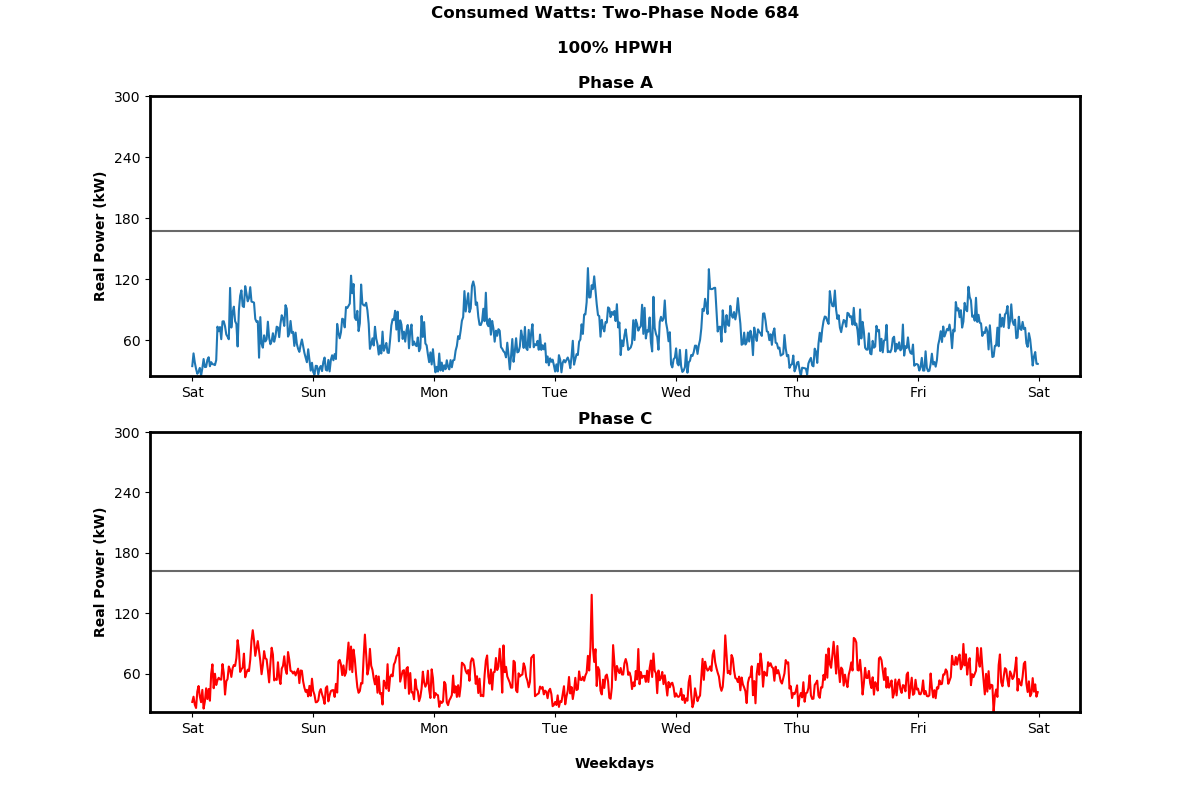
\includegraphics[width=1.1\columnwidth]{Pictures/hundred_two_phase_684_power.png}
    \caption{ }
    %\label{fig:temp_data}
\end{figure}

\newpage

\begin{figure}[H]
    \centering
    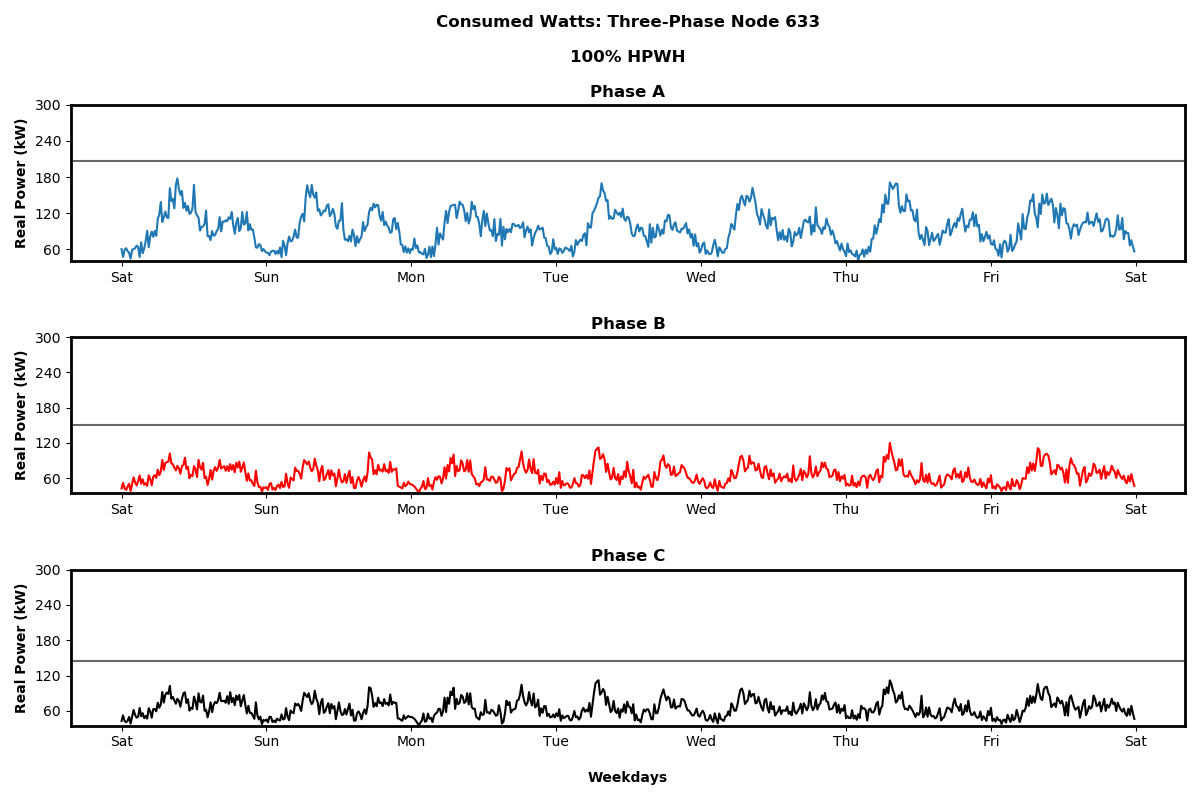
\includegraphics[width=1.1\columnwidth]{Pictures/hundred_three_phase_633_power.png}
    \caption{ }
    %\label{fig:temp_data}
\end{figure}



// ==================================================================================

\begin{figure}[H]
    \centering
    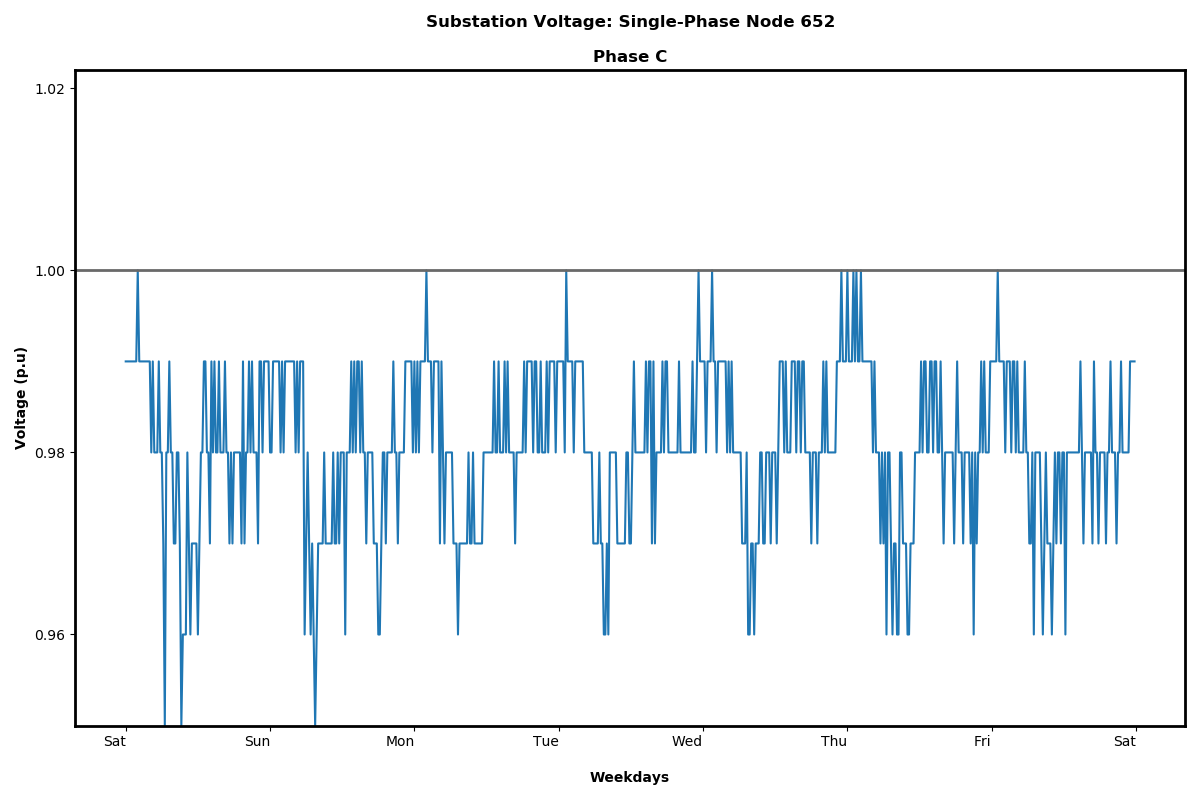
\includegraphics[width=1.1\columnwidth]{Pictures/basecase_single_phase_652_volt.png}
    \caption{ }
    %\label{fig:basecase_pow}
\end{figure}

\newpage

\begin{figure}[H]
    \centering
    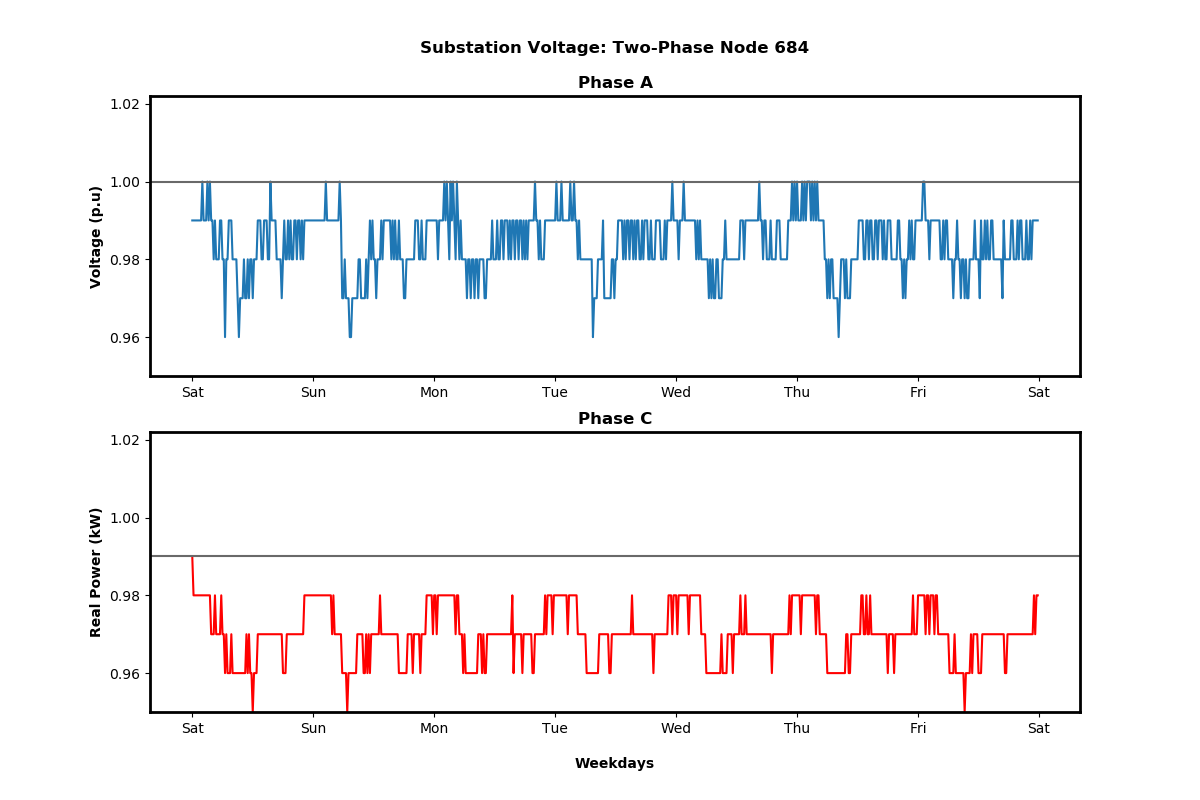
\includegraphics[width=1.1\columnwidth]{Pictures/basecase_two_phase_684_volt.png}
    \caption{ }
    %\label{fig:temp_data}
\end{figure}

\newpage

\begin{figure}[H]
    \centering
    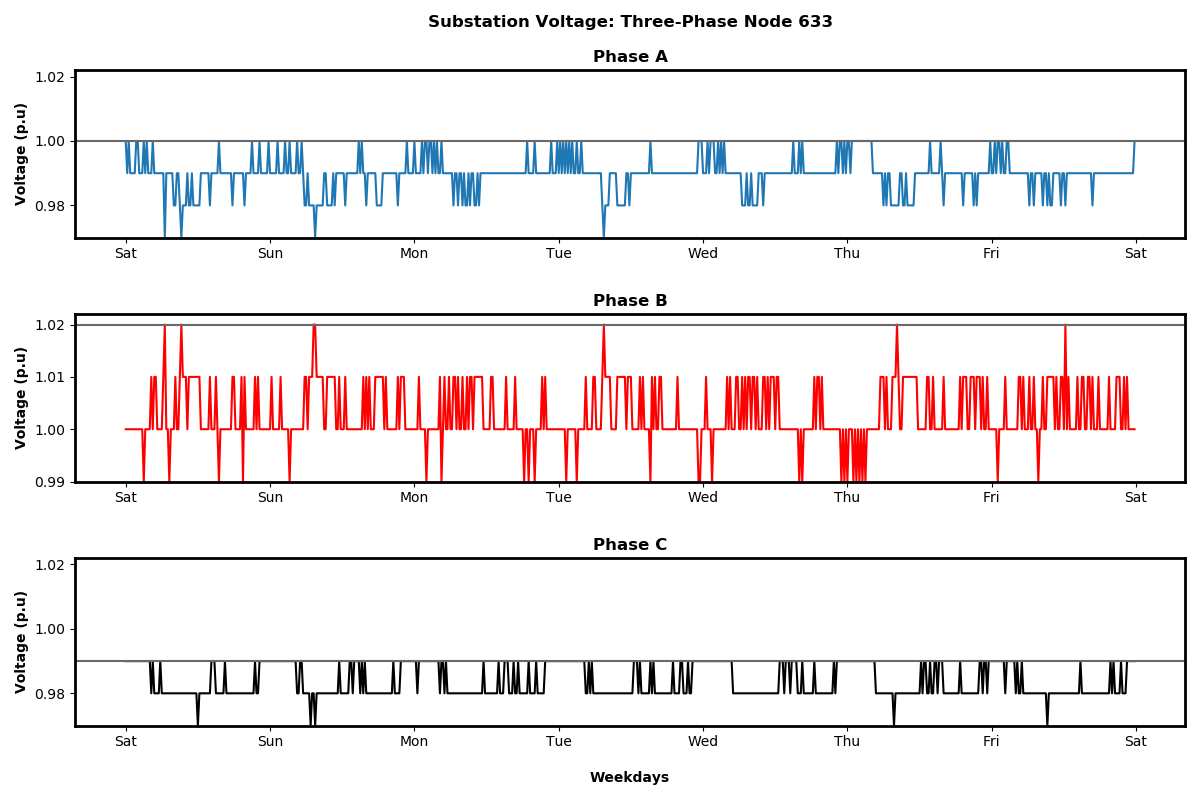
\includegraphics[width=1.1\columnwidth]{Pictures/basecase_three_phase_633_volt.png}
    \caption{ }
    %\label{fig:temp_data}
\end{figure}
\newpage


\begin{figure}[H]
    \centering
    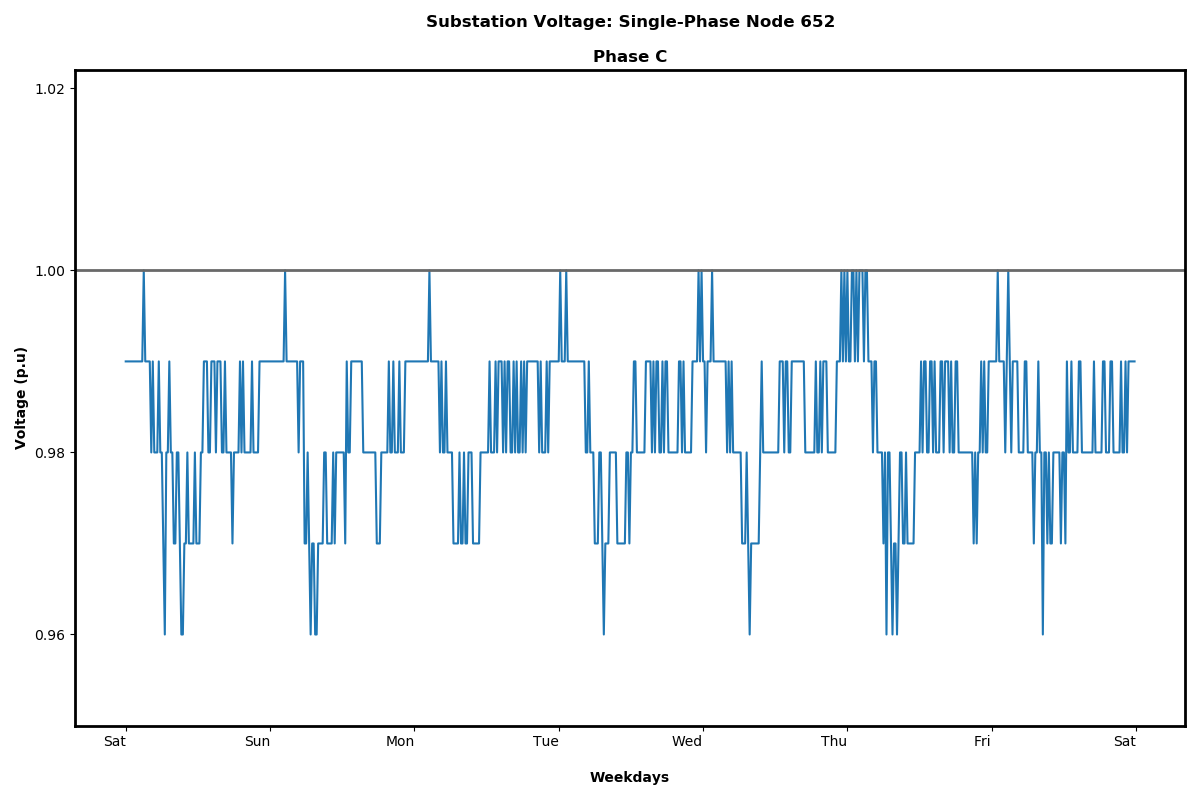
\includegraphics[width=1.1\columnwidth]{Pictures/twenty_single_phase_652_volt.png}
    \caption{ }
    %\label{fig:basecase_pow}
\end{figure}

\newpage

\begin{figure}[H]
    \centering
    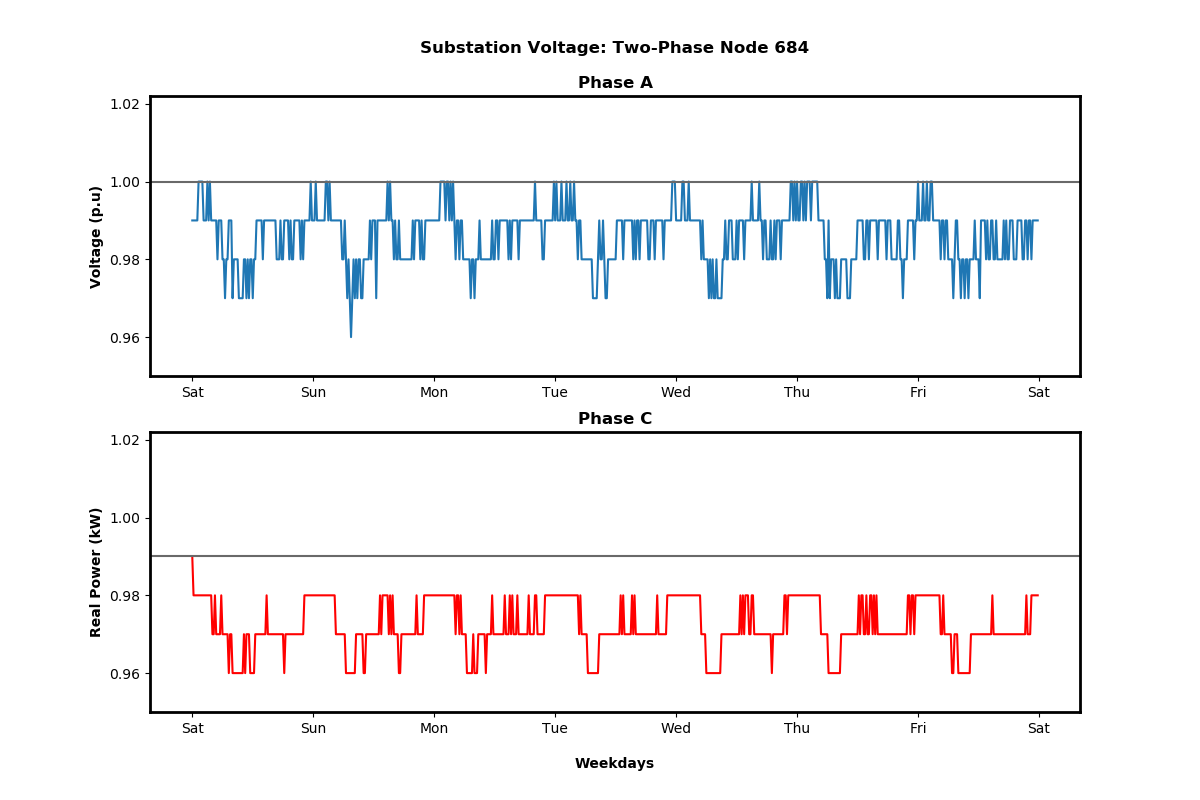
\includegraphics[width=1.1\columnwidth]{Pictures/twenty_two_phase_684_volt.png}
    \caption{ }
    %\label{fig:temp_data}
\end{figure}

\newpage

\begin{figure}[H]
    \centering
    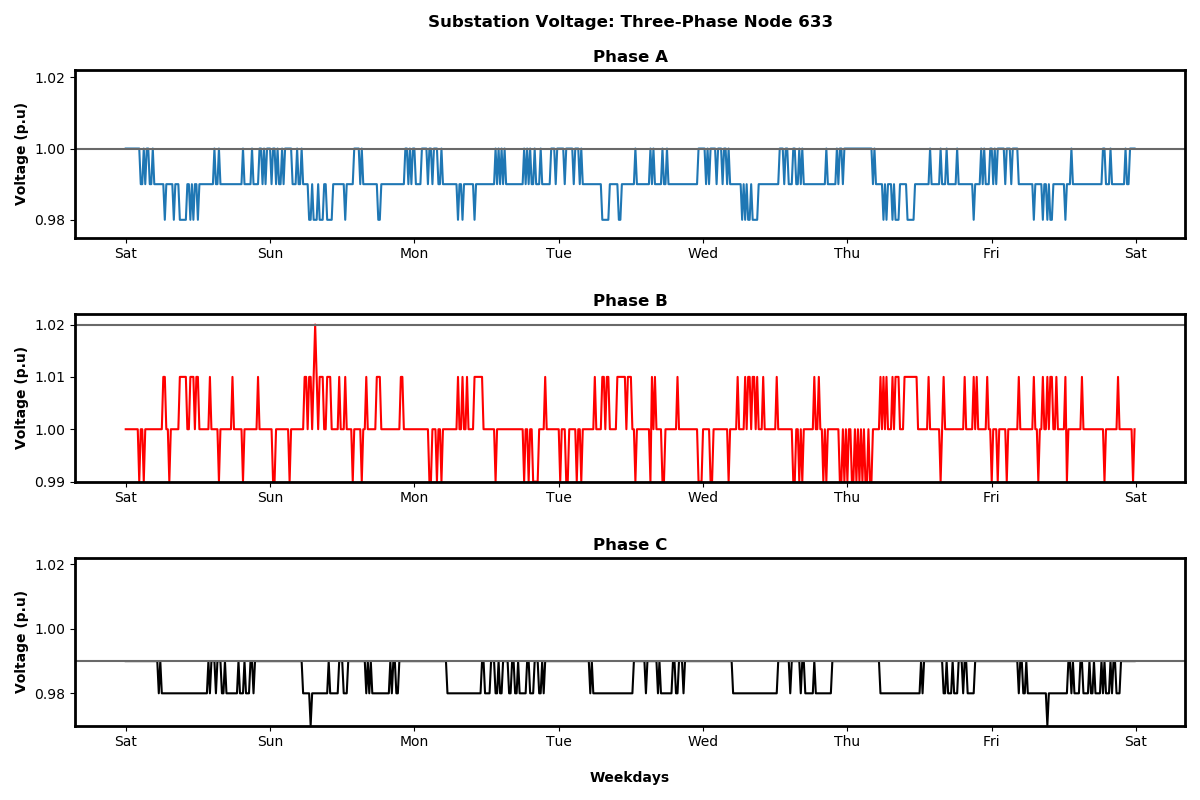
\includegraphics[width=1.1\columnwidth]{Pictures/twenty_three_phase_633_volt.png}
    \caption{ }
    %\label{fig:temp_data}
\end{figure}




\begin{figure}[H]
    \centering
    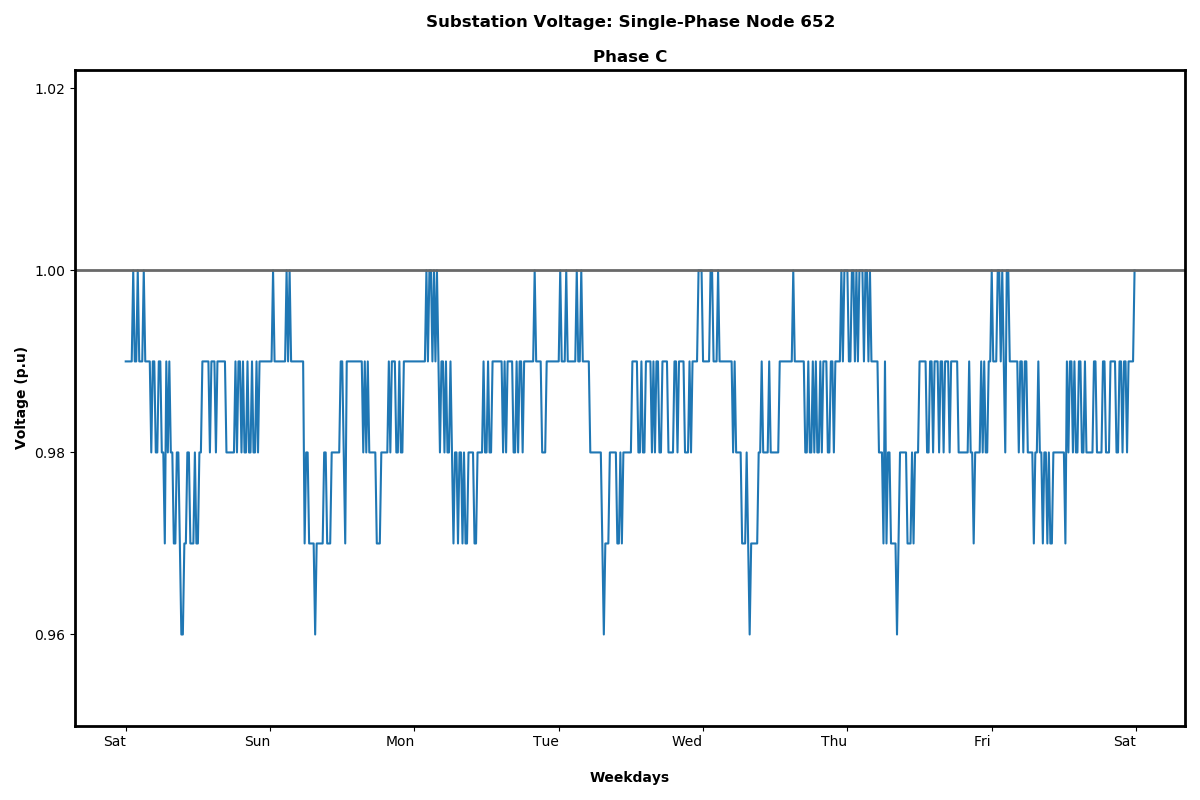
\includegraphics[width=1.1\columnwidth]{Pictures/fourty_single_phase_652_volt.png}
    \caption{ }
    %\label{fig:basecase_pow}
\end{figure}

\newpage

\begin{figure}[H]
    \centering
    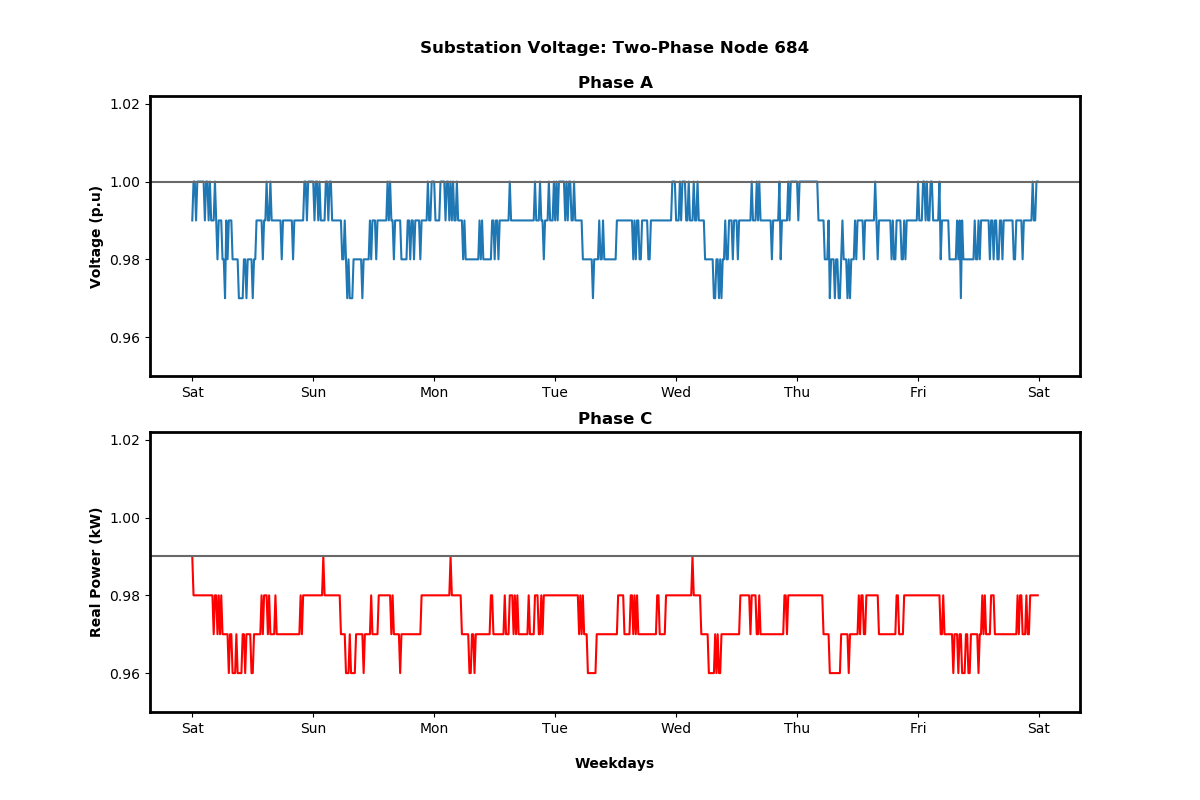
\includegraphics[width=1.1\columnwidth]{Pictures/fourty_two_phase_684_volt.png}
    \caption{ }
    %\label{fig:temp_data}
\end{figure}

\newpage

\begin{figure}[H]
    \centering
    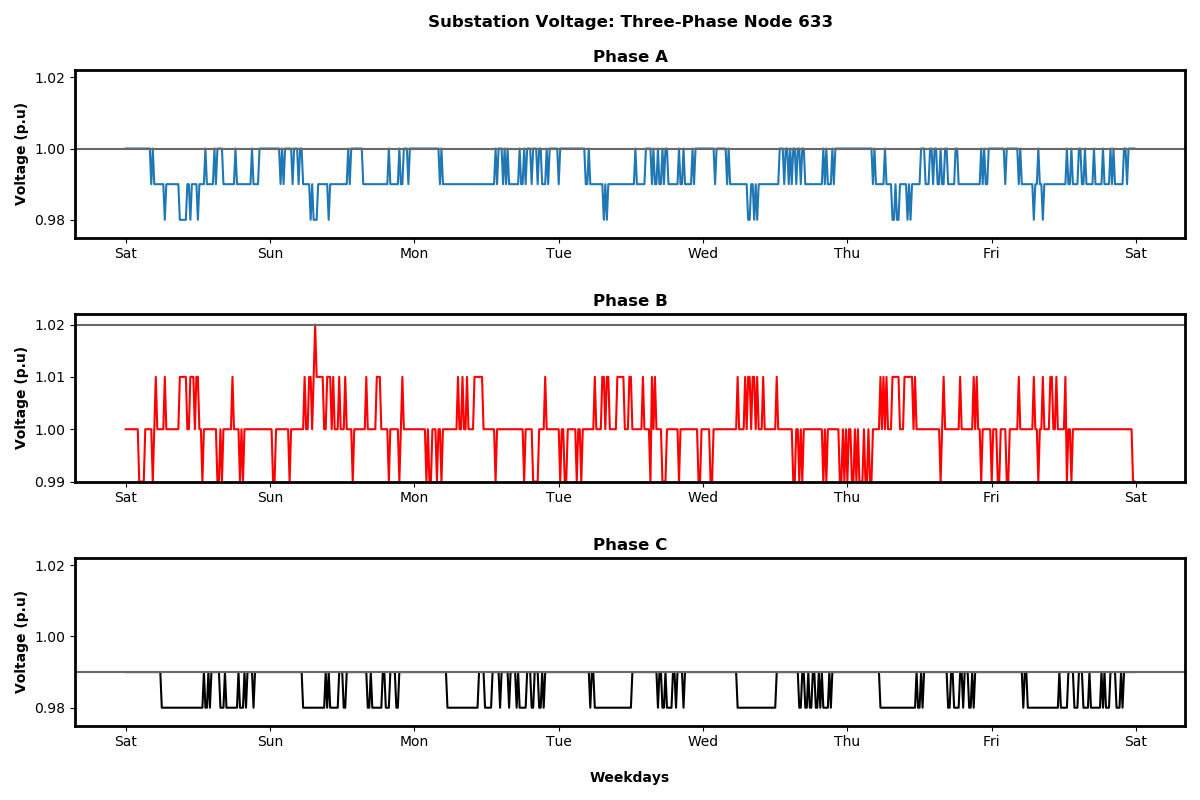
\includegraphics[width=1.1\columnwidth]{Pictures/fourty_three_phase_633_volt.png}
    \caption{ }
    %\label{fig:temp_data}
\end{figure}

\newpage



\begin{figure}[H]
    \centering
    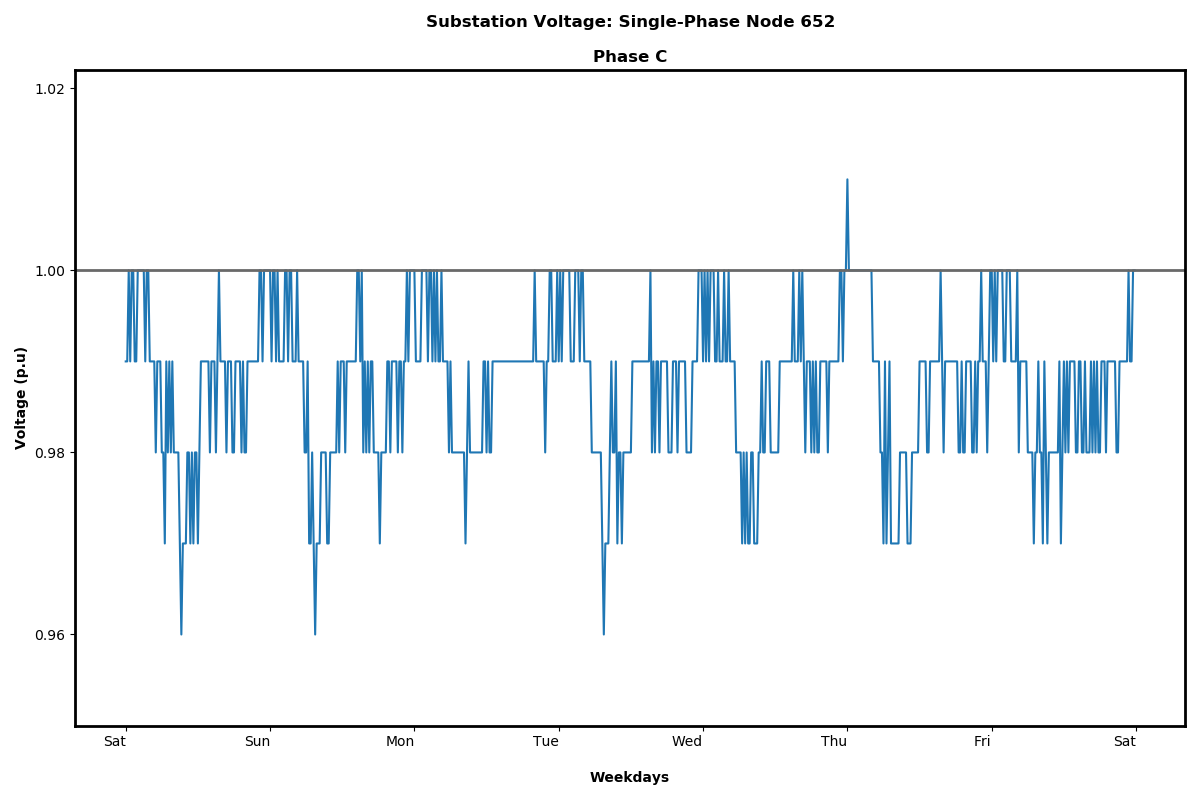
\includegraphics[width=1.1\columnwidth]{Pictures/sixty_single_phase_652_volt.png}
    \caption{ }
    %\label{fig:basecase_pow}
\end{figure}

\newpage

\begin{figure}[H]
    \centering
    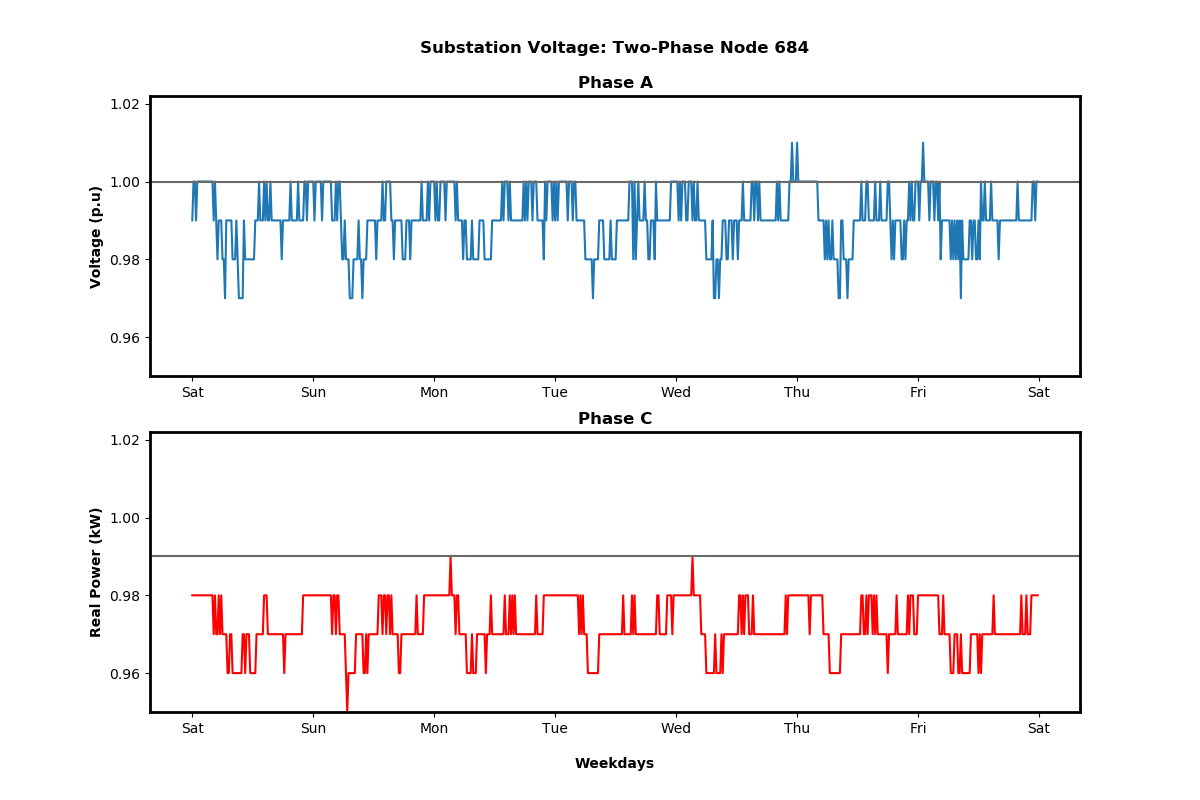
\includegraphics[width=1.1\columnwidth]{Pictures/sixty_two_phase_684_volt.png}
    \caption{ }
    %\label{fig:temp_data}
\end{figure}

\newpage

\begin{figure}[H]
    \centering
    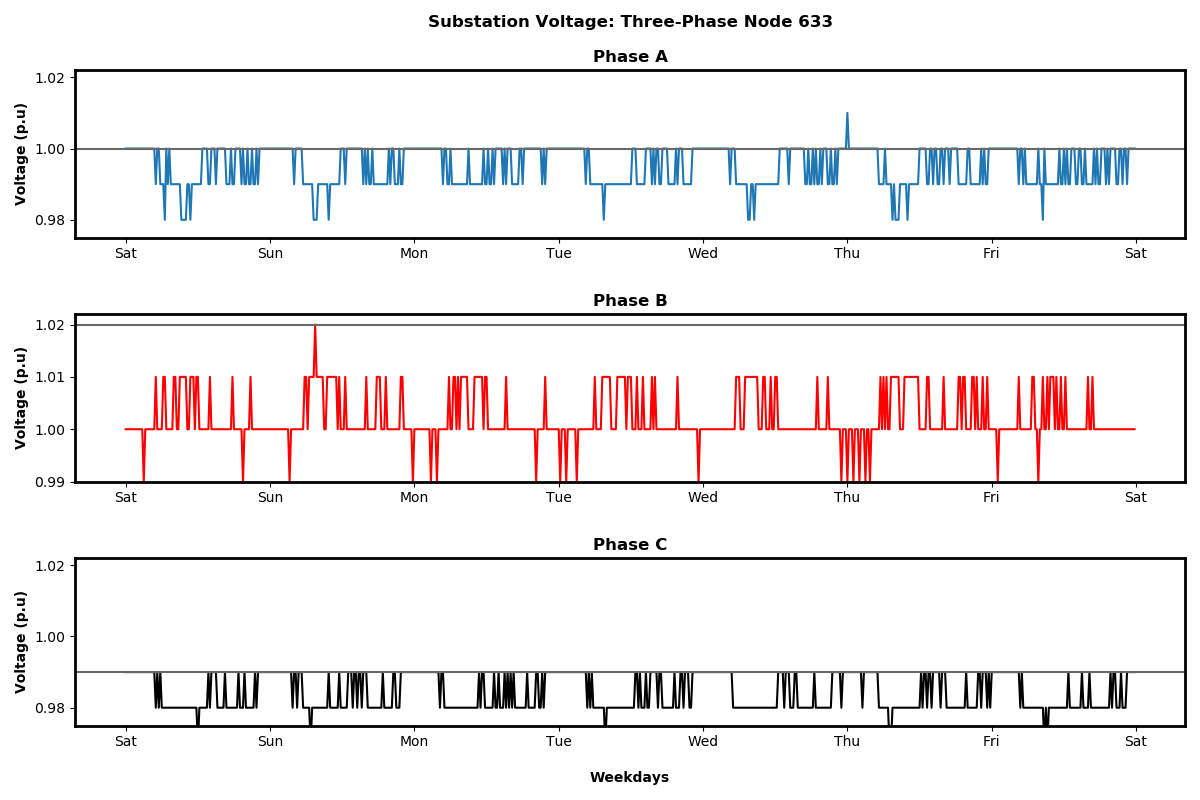
\includegraphics[width=1.1\columnwidth]{Pictures/sixty_three_phase_633_volt.png}
    \caption{ }
    %\label{fig:temp_data}
\end{figure}
\newpage





\begin{figure}[H]
    \centering
    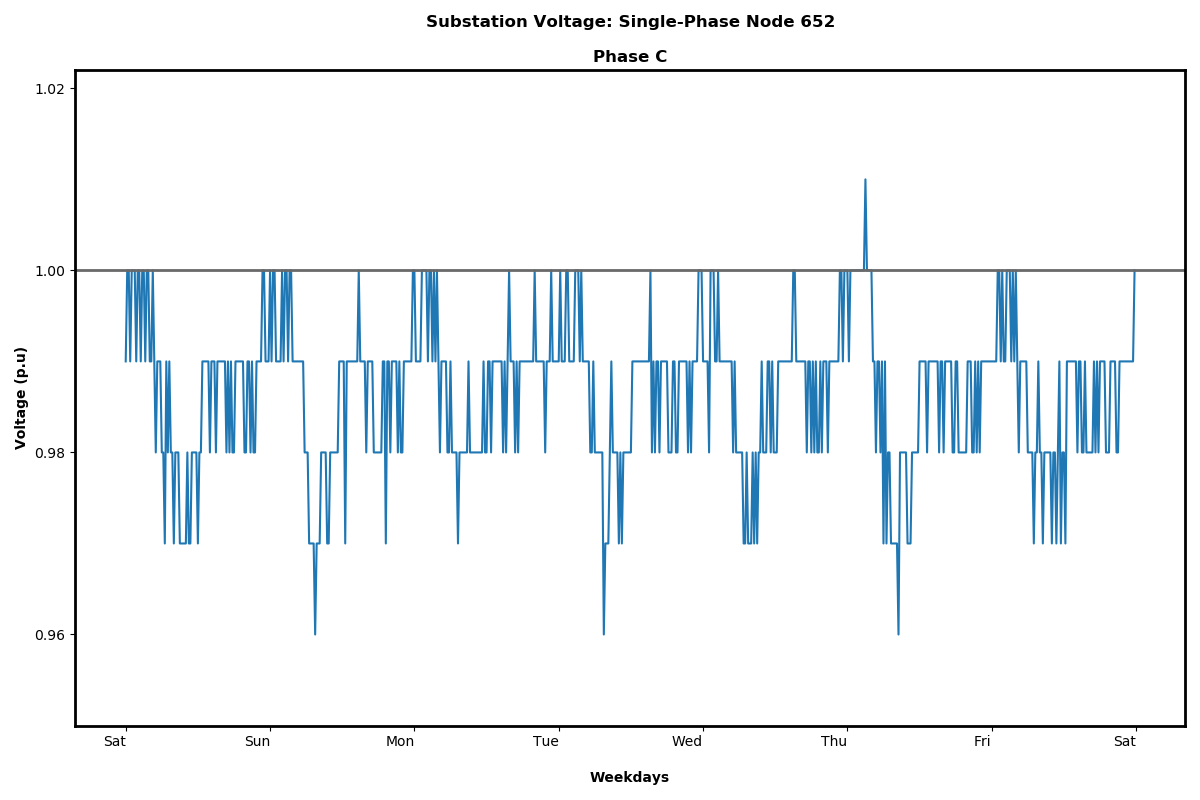
\includegraphics[width=1.1\columnwidth]{Pictures/eighty_single_phase_652_volt.png}
    \caption{ }
    %\label{fig:basecase_pow}
\end{figure}

\newpage

\begin{figure}[H]
    \centering
    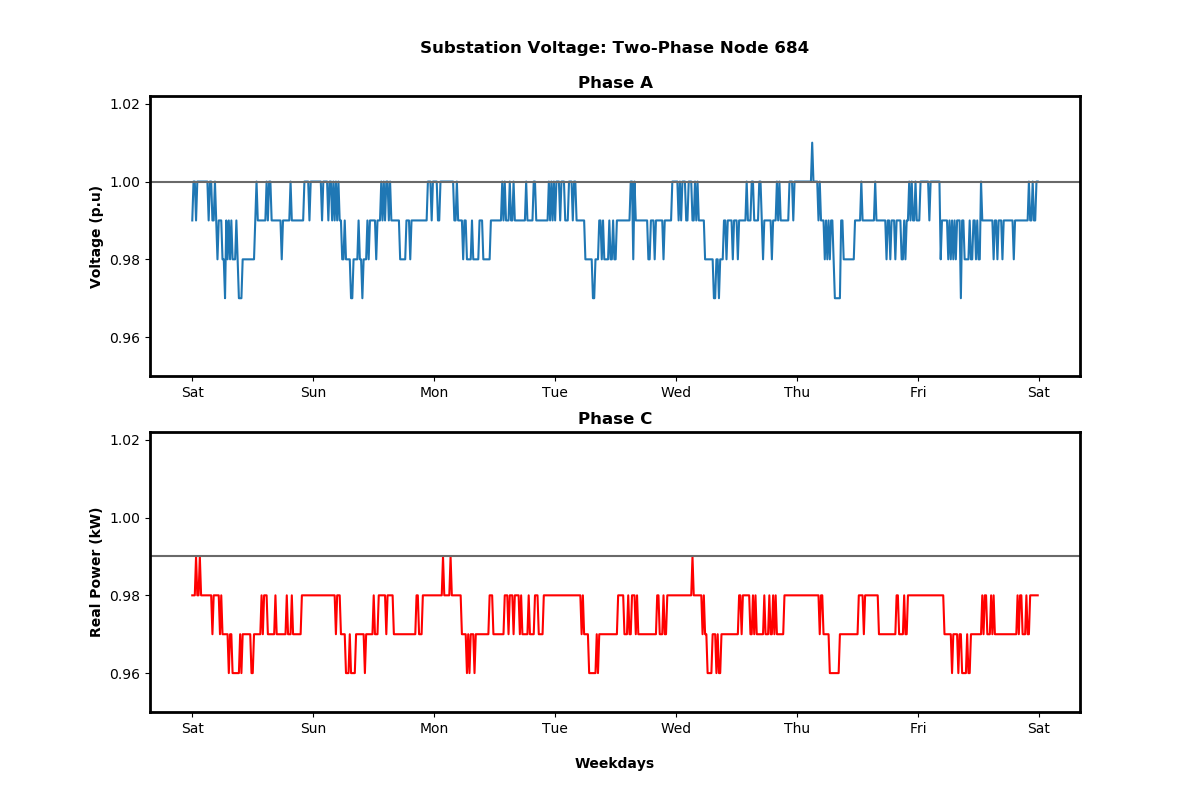
\includegraphics[width=1.1\columnwidth]{Pictures/eighty_two_phase_684_volt.png}
    \caption{ }
    %\label{fig:temp_data}
\end{figure}

\newpage

\begin{figure}[H]
    \centering
    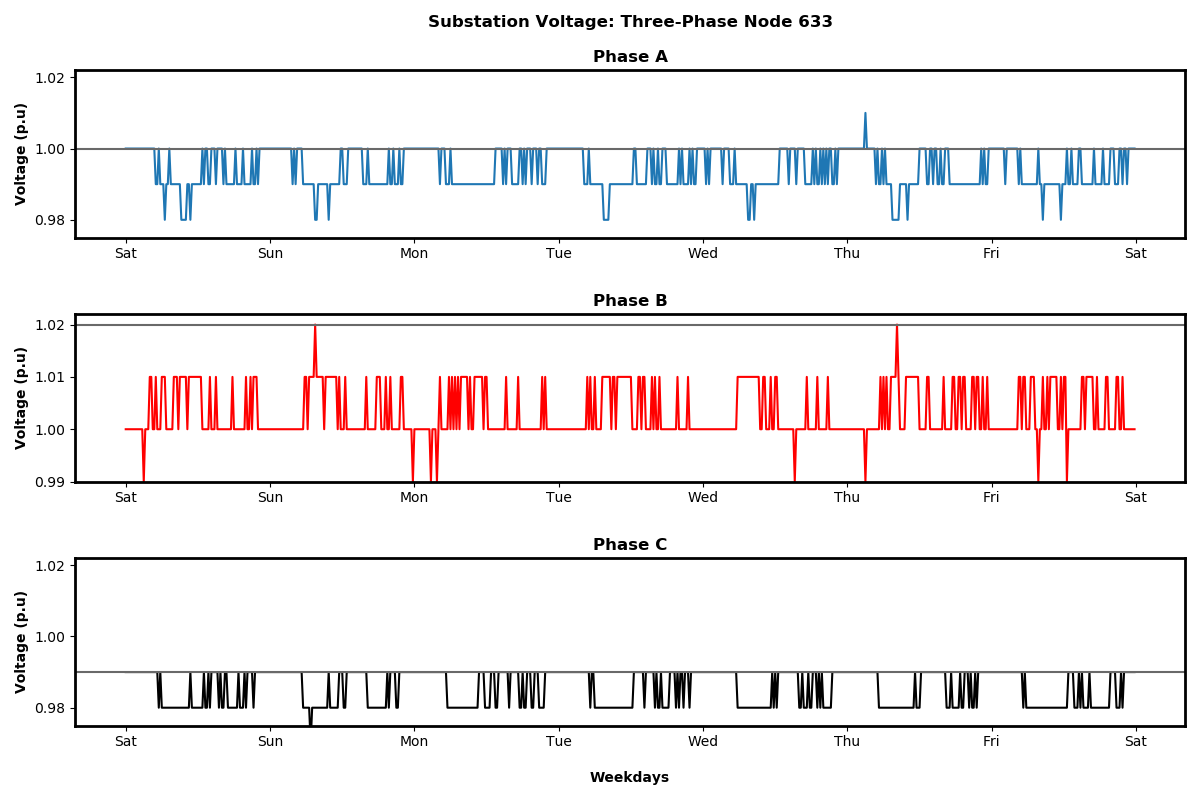
\includegraphics[width=1.1\columnwidth]{Pictures/eighty_three_phase_633_volt.png}
    \caption{ }
    %\label{fig:temp_data}
\end{figure}

\newpage





\begin{figure}[H]
    \centering
    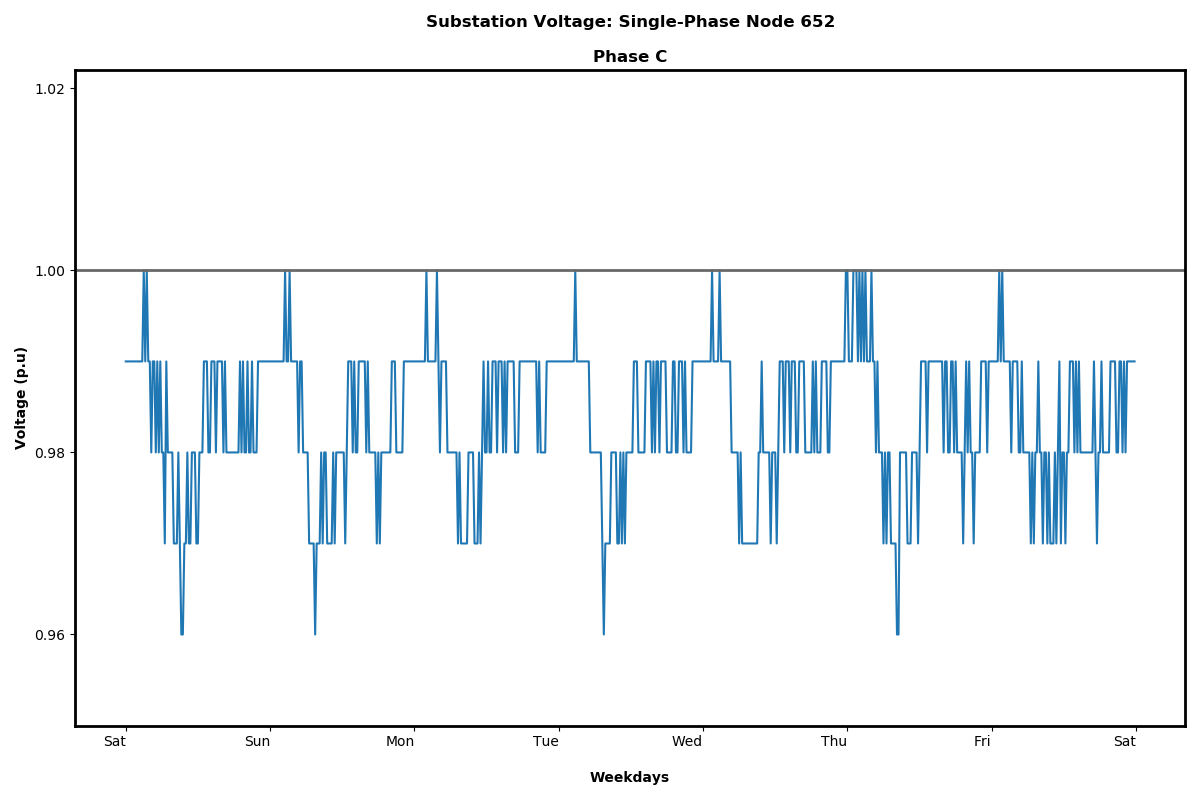
\includegraphics[width=1.1\columnwidth]{Pictures/hundred_single_phase_652_volt.png}
    \caption{}
    %\label{fig:basecase_pow}
\end{figure}

\newpage

\begin{figure}[H]
    \centering
    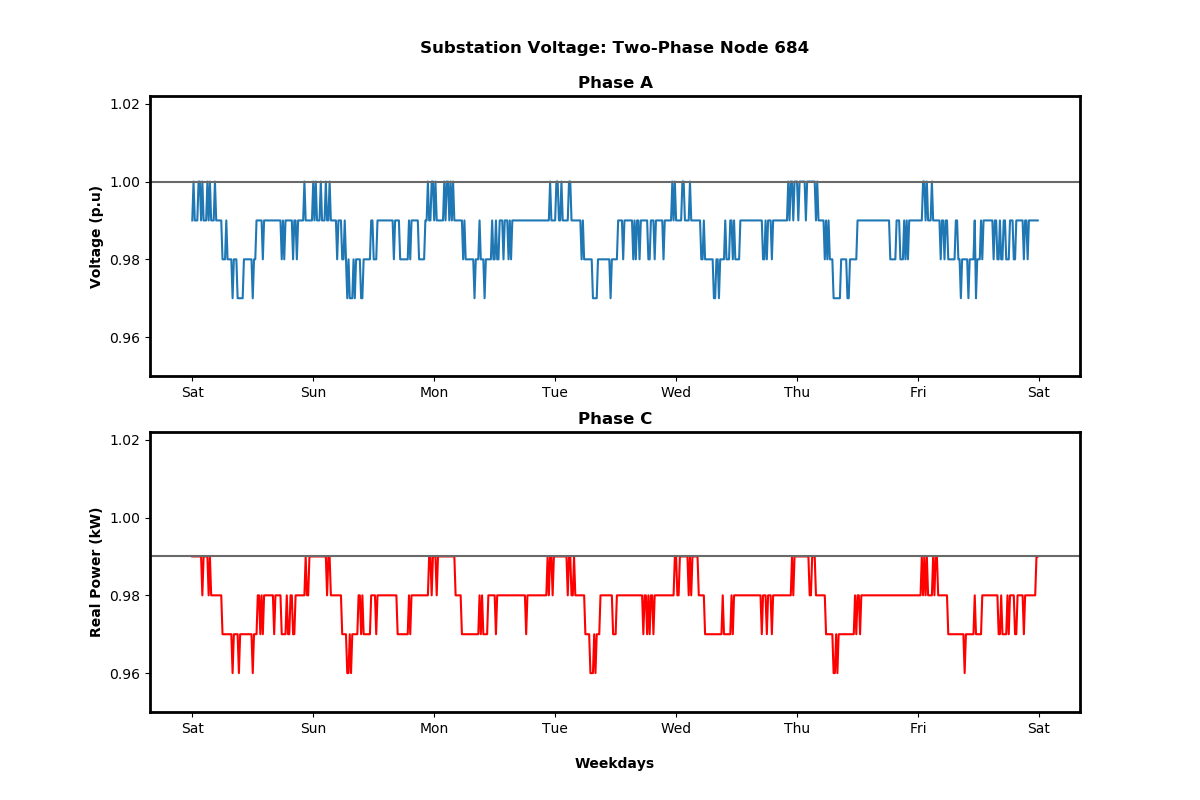
\includegraphics[width=1.1\columnwidth]{Pictures/hundred_two_phase_684_volt.png}
    \caption{}
    %\label{fig:temp_data}
\end{figure}

\newpage

\begin{figure}[H]
    \centering
    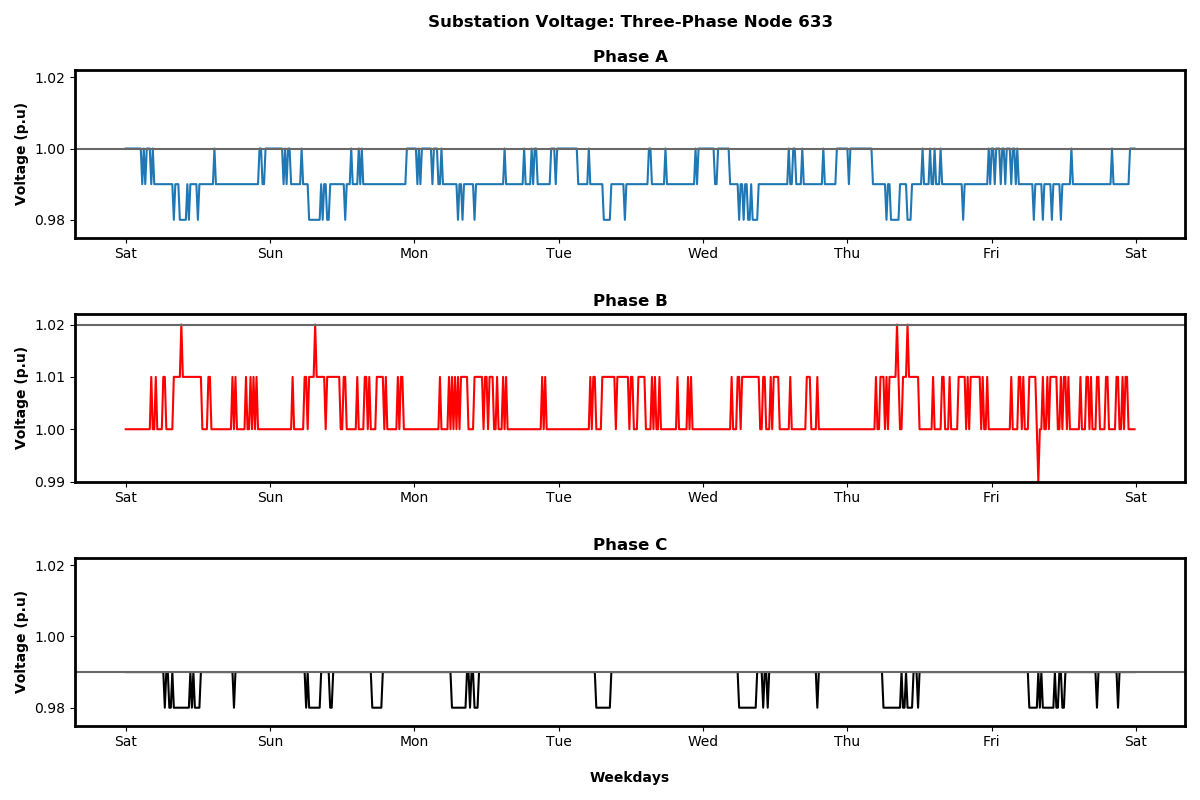
\includegraphics[width=1.1\columnwidth]{Pictures/hundred_three_phase_633_volt.png}
    \caption{}
    %\label{fig:temp_data}
\end{figure}

\newpage

% \section{GridAPPS-D}

% \subsection{Converting GLM files to CIM Files}

% GridAPPS-D uses cim file format. In our case, we have several glm file models (GridLAB-D) that we want to convert to CIM file format (GridAPPS-D format). This process can be done by using scripts within GridAPPS-D repository. 

% Some issues exist, however, when converting from GLM files to CIM files. These issues lie within the ``house objects'' in GridLAB-D. The conversion scripts will convert each ``house object'' to a ``triplex load''. This might affect the model overall as we use these ``house objects'' to provide weather environment for the \gls{hpwh}. 

% This is not a big deal and I believe we can easily figure a work around that by simply remove the ``house objects''. Keep in mind that the ``house objects'' are linked with other objects. So a model reconfiguration might be needed. The other workaround is to use the IEEE 13 node feeder as it is within GridAPPS-D, then use ``insertDER.py'' script to add the required loads and triplex configurations.

% \subsubsection{Questions}
% \begin{itemize}
% \item In the GLM file, we use several load profiles that are read by the triplex load objects. If we convert the GLM file to a CIM file, can we still use these load profiles?
% \end{itemize}
